\tableofcontents




%\part{Alku}
\chapter{Esipuhe}

%%%%%%%%%%%%%%%%%%%%%%%%%%%%%%%%%%%%%%%%%%%%%%%%%%%%%%%%%%%%%%%%%%%%%%%%%%%%%%%%
%%%%  /usr/share/doc/texlive-fonts-extra-doc/fonts/arev/mathtesty.tex

% mathtesty.tex, by Stephen Hartke 20050522
% based on mathtestx.tex in the mathptmx package
% and symbols.tex by David Carlisle

Matematiikka tarjoaa työkaluja asioiden jäsentämiseen, päättelyyn ja mallintamiseen. Alasta riippuen käsittelemme matematiikassa erilaisia \textbf{objekteja}: Geometriassa tarkastelemme tasokuvioita ja kolmiulotteisia rakenteita. Algebra tutkii lukujen ja funktioiden ominaisuuksia. Todennäköisyyslaskenta arvioi erilaisten tapausten ja tilanteiden mahdollisuuksia ja riskejä. Matemaattinen analyysi (kurssit 7,8 ja 10) tutkii funktioita ja niiden muuttumista.

Jokaiseen tarkastelukohteeseen liitetään myös niille ominaisia \textbf{operaatioita}. Tämä kurssi käsittelee lähinnä lukuja ja niiden operaatioita, joita \textbf{laskutoimituksiksi} kutsutaan. Kirjan ensimmäisessä osassa käsittelemme luvun käsitteen, yleisimmät lukutyypit ja lukujen tavallisimman laskutoimitukset.

\section*{Sananen kirjasta}

Tulimme, kirjoitimme, voitimme.

\section*{Tekijöiden kommentit}

\todo{Miten olisi lyhyt kommentti tai lainaus jokaiselta tekijältä? Jotain yleviä mietteitä kirjasta, rohkaisevia tai nasevia kommentteja lukijalle, alku- tai loppukevennyksiä tai jotain randomia}

\begin{tabular}{cc} 
	\begin{tabular}{c}
	 \textbf{Lauri Hellsten}
	\\ 
	kommentti1 \end{tabular}
&
	\begin{tabular}{c}
	 \textbf{Niko Ilomäki}
	\\ 
	kommentti2 \end{tabular}
\\
	\begin{tabular}{c}
	 \textbf{Tero Keinänen}
	\\ 
	kommentti3 \end{tabular}
&
	\begin{tabular}{c}
	 \textbf{Vesa Linja-aho}
	\\ 
	kommentti4 \end{tabular}
\\
	\begin{tabular}{c}
	 \textbf{Ossi Mauno}
	\\ 
	kommentti1 \end{tabular}
&
	\begin{tabular}{c}
	 \textbf{Joonas Mäkinen}
	\\ 
	kommentti2 \end{tabular}
\\
	\begin{tabular}{c}
	 \textbf{Matti Pajunen}
	\\ 
	kommentti3 \end{tabular}
&
	\begin{tabular}{c}
	 \textbf{Pekka Peura}
	\\ 
	kommentti4 \end{tabular}
\\
	\begin{tabular}{c}
	 \textbf{Annika Piiroinen}
	\\ 
	kommentti1 \end{tabular}
&
	\begin{tabular}{c}
	 \textbf{Kaisa Pohjonen}
	\\ 
	kommentti2 \end{tabular}
\\
	\begin{tabular}{c}
	 \textbf{Antti Rasila}
	\\ 
	kommentti3 \end{tabular}
&
	\begin{tabular}{c}
	 \textbf{Johanna Rämö}
	\\ 
	kommentti4 \end{tabular}		
\\
	\begin{tabular}{c}
	 \textbf{Annika Piiroinen}
	\\ 
	kommentti1 \end{tabular}
&
	\begin{tabular}{c}
	 \textbf{Kaisa Pohjonen}
	\\ 
	kommentti2 \end{tabular}
\\
	\begin{tabular}{c}
	 \textbf{Antti Rasila}
	\\ 
	kommentti3 \end{tabular}
&
	\begin{tabular}{c}
	 \textbf{Johanna Rämö}
	\\ 
	kommentti4 \end{tabular}
	\\
	\begin{tabular}{c}
	 \textbf{Juha Sointu}
	\\ 
	kommentti1 \end{tabular}
&
	\begin{tabular}{c}
	 \textbf{Tommi Sottinen}
	\\ 
	kommentti2 \end{tabular}
\\
	\begin{tabular}{c}
	 \textbf{Jarno Talponen}
	\\ 
	kommentti3 \end{tabular}
&
	\begin{tabular}{c}
	 \textbf{Topi Talvitie}
	\\ 
	kommentti4 \end{tabular}
\\
	\begin{tabular}{c}
	 \textbf{Sampo Tiensuu}
	\\ 
	kommentti3 \end{tabular}
&
	\begin{tabular}{c}
	 \textbf{Ville Tilvis}
	\\ 
	kommentti4 \end{tabular}
	
	  
\end{tabular} 

\section*{Kiitämme}
\begin{itemize}
\item Metropolia
\item TEK
\item Senja Larsen
\item Kebab Pizza Service
\end{itemize}

%%%%%%%%%%%%%%%%%%%%%%%%%%%%%%%%%%%%%%%%%%%%%%%%%%%%%%%%%%%%%%%%%%%%%%%%%%%%%%%%
%%%% /usr/share/doc/texlive-doc-en/fonts/free-math-font-survey/source/textfragment.tex







%%% Local Variables: 
%%% mode: latex
%%% End: 


\part{Luvut ja laskutoimitukset}
    \chapter{Numerot ja luvut}

Ihmisellä ja muilla eläimillä on luonnostaan matemaattisia taitoja. Monet niistä, esimerkiksi lukumäärien laskeminen, ovat yllättävän monimutkaisia kognitiivisia prosesseja, jotka kehittyvät lapsuudessa – toisilla aiemmin, toisilla myöhemmin. Kaikki koulussa opeteltava peruslaskento ja myös matematiikka tieteen alana rakentavat tämän biologisen osaamisen päälle. Laskeminen itsessään on vain yksi matematiikan osa-alue, eikä kaikki matematiikka ole laskemista.

\sivulaatikko{Huom.! laskea (lukumäärä) englanti count ruotsi \_ /n
laskea (laskutoimitus) englanti calculate , ruotsi \_}

Hyvin olennaisena kehitysaskeleena niin yksilön matemaattiselle ajattelulle kuin yhteiskunnallekin on ollut luonnollisen kielen tavoin kyky merkitä lukumäärien laskemista ja muuta matemaattista pohdintaa kirjalliseen muotoon. On olemassa hyvin monia erilaisia tapoja merkitä lukumääriä. Helpoin tapa ja yksinkertaisin tapa on käyttää vain yhtä samaa merkkiä ja toistaa sitä:

\missingfigure{Piirrettynä "tukkimiehen kirjanpitoa" ja  vertaus arabialaisilla numeroilla}

Käytettävissä olevien merkkien määrää voidaan lisätä, jolloin suuria lukuja voidaan kirjoittaa lyhyemmin. Tämä vastaa myös luonnollisten kielten tilannetta: Suomen kielen aakkosiin kuuluu 29 kirjainta, joista sanat muodostetaan. Sanat voivat olla kuinka pitkiä vain kahdesta kirjaimesta ylöspäin. Mandariinikiinassa sen sijaan käytetään omaa piirrosmerkkiä jokaiselle sanalle. Merkkejä täytyy osata 29 sijaan tuhansia, mutta jokaisen sanan voi kirjoittaa lyhyesti.

Matematiikassa erilaisista numeromerkeistä tai yksinkertaisesti numeroista muodostetaan lukuja yhdistelemällä niitä sopivasti erilaisten paikkajärjestelmien mukaan. Esimerkiksi antiikin Roomassa käytössä olivat numeromerkit I, V, X, L, C , D ja M. Niiden numeroiden vastaavuudet meidän käyttämiimme lukuarvoihin ovat seuraavat:
I=1
V=5
X=10
L=50
C=100
D=500
M=1 000
Huomaa, että suuri osa roomalaisista numeromerkeistä ovat jo itsessään arvoltaan niin suuria, että me tarvitsemme niiden nykyilmaisuun monta merkkiä! Nollaa roomalaisissa numeroissa ei ole, ja tiettävästi tuhatta suurempia arvoja esittäviä numeromerkkejä merkkejä otettiin käyttöön vasta keskiajalla. 
Lukuja koostetaan näistä merkeistä siten, että merkit kirjoitetaan peräkkäin pääasiassa laskevassa järjestyksessä ja niiden numeroarvot lasketaan yhteen. Jos arvoltaan pienempi numeromerkki (korkeintaan yksi) edeltää suurempaa, pienempi vähennetään suuremmasta ennen yhteenlaskun jatkamista. 

Luvut $134$ ja $413$ eivät ole sama luku; saamme eri lukuja, kun numeroita yhdistellään eri tavoin.

\begin{esimerkki}
III=1+1+1=3
IX=10-1=9
XII=10+1+1=12
XIX=10-1+10=19
CDX=500-100+10=410
MCMD=1 000+1 000-100+500
\end{esimerkki}


\laatikko{Länsimaisessa traditiossa käytössämme on kymmenen numeromerkkiä: 0, 1, 2, 3, 4, 5, 6, 7, 8 ja 9. Näitä kutsutaan alkuperänsä mukaan hindu-arabialaisiksi numeroiksi.}

Yksittäisellä numeromerkillä ei kuitenkaan ole vielä matematiikassa tarvittavaa lukuarvoa, vaan luvut rakennetaan yhdistelemällä numeroita.

\begin{esimerkki}
Luku \[715531\] koostuu numeroista 7, 1, 5, 5, 3 ja 1.
\end{esimerkki}



\sivulaatikko{Englannin kielen sana \textit{number} voi viitata sekä numeroon että lukuun. Sana \textit{digit} tarkoittaa pelkästään yhtä numeromerkkiä. Ruotsiksi luku on \textit{tal}, lukumäärä \textit{antal} ja numeroa tai lukumäärää tarkoittamatonta numeroyhdistelmää kuvaa suomen kielen tapaan sana \textit{nummer}.}



postinumero, puhelinnumero!


\begin{esimerkki}
Selitys kymmenjärjestelmästä, kymmenet, sadat, tuhannet, ...
\[20661,43\]
\end{esimerkki}

\sivulaatikko{Kielioppihuomautuksia: 1) Tuhaterottimena käytetään välilyöntiä, ei pilkkua tai pistettä. 2) Suomessa on käytössä desimaalipilkku, ei -piste! Yhdysvaltalaiset ovat suunnitelleet laskimesi.}


\section{Jos tämä on matematiikkaa, miksi käytämme kirjaimia?}

Numeroita kuvaavat merkit ovat mielivaltaisia symboleita. Lukujakin edustamaan päädytään joskus käyttämään jotakin lyhennysmerkintää

yleisyys

suuruus, yhtäsuuruusmerkintä, eri suuret

$x=2$
-> $2=x$
symbolit, muuttujat, alkiot, kreikkalaisia...

\sivulaatikko{Painotekstissä kirjaimella merkityt muuttujat kirjoitetaan \textit{kursiivilla} ja aina saman arvon saavat matemaattiset vakiot kuten $\pi$ pystyyn.}

\section{Paikka- lukujärjestelmät}





Erilaisilla luvuilla voidaan suorittaa erilaisia laskutoimituksia. Seuraavissa luvuissa esitellään ja käydään läpi lukiomatematiikassa ja mahdollisissa jatko-opinnoissa käytettäviä lukujoukkoja ja tavallisimmat laskutoimitukset.

    \chapter{Luonnolliset luvut}

(Joonas jatkaa tästä vielä!)

Suomen kielen verbi 'laskea' voi tarkoittaa matematiikassa kahta eri asiaa: lukumäärien laskemista ja laskutoimitusten suorittamista.

\laatikko{laskea (lukumäärä) englanti count ruotsi \_ /n
laskea (laskutoimitus) englanti calculate , ruotsi \_}

Ihmisellä ja muilla eläimillä on luonnostaan matemaattisia taitoja. Monet niistä, esimerkiksi lukumäärien laskeminen, ovat yllättävän monimutkaisia kognitiivisia prosesseja, jotka kehittyvät lapsuudessa – toisilla aiemmin, toisilla myöhemmin. Kaikki koulussa opeteltava peruslaskento ja myös matematiikka tieteen alana rakentavat tämän biologisen osaamisen päälle. Laskeminen itsessään on vain yksi matematiikan osa-alue, eikä kaikki matematiikka ole laskemista. Huomaa, että suomen kielen verbillä laskea tarkoitetaan sekä lukumäärien laskemista (engl. counting) että lukujen laskutoimitusten suorittamista (engl. calculating).

Hyvin olennaisena kehitysaskeleena niin yksilön matemaattiselle ajattelulle kuin yhteiskunnallekin on ollut luonnollisen kielen tavoin kyky merkitä lukumäärien laskemista ja muuta matemaattista pohdintaa kirjalliseen muotoon.  On olemassa hyvin monia erilaisia tapoja merkitä lukumääriä. Helpoin tapa ja yksinkertaisin tapa on käyttää vain yhtä samaa merkkiä ja toistaa sitä. Jos

käytettävissä olevien merkintöjä määrää voidaan lisätä, jolloin suuria lukuja voidaan kirjoittaa lyhyemmin. Tämä vastaa myös luonnollisten kielten tilannetta: Suomen kielen aakkosiin kuuluu 29 kirjainta, joista sanat muodostetaan. Sanat voivat olla kuinka pitkiä vain kahdesta kirjaimesta ylöspäin. Kiinassa sen sijaan käytetään omaa piirrosmerkkiä jokaiselle sanalle. Merkkejä täytyy osata 29 sijaan tuhansia, mutta jokaisen sanan voi kirjoittaa lyhyesti. 
Matematiikassa erilaisista numeromerkeistä tai yksinkertaisesti numeroista muodostetaan lukuja yhdistelemällä niitä sopivasti erilaisten paikkajärjestelmien mukaan. Esimerkiksi antiikin Roomassa käytössä olivat numeromerkit I, V, X, L, C , D ja M. Niiden numeroiden vastaavuudet meidän käyttämiimme lukuarvoihin ovat seuraavat:
I=1
V=5
X=10
L=50
C=100
D=500
M=1 000
Huomaa, että suuri osa roomalaisista numeromerkeistä ovat jo itsessään arvoltaan niin suuria, että me tarvitsemme niiden nykyilmaisuun monta merkkiä! Nollaa roomalaisissa numeroissa ei ole, ja tiettävästi tuhatta suurempia arvoja esittäviä numeromerkkejä merkkejä otettiin käyttöön vasta keskiajalla. 
Lukuja koostetaan näistä merkeistä siten, että merkit kirjoitetaan peräkkäin pääasiassa laskevassa järjestyksessä ja niiden numeroarvot lasketaan yhteen. Jos arvoltaan pienempi numeromerkki (korkeintaan yksi) edeltää suurempaa, pienempi vähennetään suuremmasta ennen yhteenlaskun jatkamista. 

    % Luonnolliset luvut esitellään nyt kokonaislukujen alussa.

% \sivulaatikko{engl. \emph{natural numbers, counting numbers} ruots. \emph{naturliga tal}}
% 
% 
% \laatikko{Luonnollisia lukuja käytetään kolmeen eri tarkoitukseen:
% 
% \begin{enumerate}
% \item Lukumäärien ilmoittamiseen (kardinaaliluvut)
% \item Järjestyksen ilmoittamiseen (ordinaaliluvut)
% \item Indeksointiin ja asioiden nimeämiseen
% \end{enumerate}
% }


% \section{Tehtäviä}
% 
% \begin{tehtava}
% 
% Onko kardinaali vai ordinaali vai indeksointi?
% 
% \end{tehtava}

\chapter{Kokonaisluvut}

Yksinkertaisimmat käyttämämme luvut ovat lukumäärien ilmaisemiseen käytetyt $0,
1, 2, 3, \ldots$. Näitä kutsutaan \emph{luonnollisiksi luvuiksi}, ja niiden
joukkoa eli kaikkia luonnollisia lukuja yhdessä merkitään symbolilla
$\mathbb{N}$. Edellä nolla määriteltiin luonnolliseksi luvuksi, mutta tästä
ei ole yhteistä sopimusta: jotkut pitävät nollaa luonnollisena lukuna ja
toiset eivät.

Luonnollisille luvuille $m$ ja $n$ on määritelty yhteenlasku $m + n$, esimerkiksi
$5 + 3 = 8$.
Luonnollisten lukujen $m$ ja $n$ kertolasku määritellään peräkkäisinä yhteenlaskuina
\[m \cdot n = \underbrace{m + m + \ldots + m}_{n\text{ kpl}} = \underbrace{n + n + \ldots + n}_{m\text{ kpl}}.\]
Nollalla kertomisen ajatellaan olevan "tyhjä yhteenlasku"\ eli nolla,
$0 \cdot m = 0$.

Luonnollisten lukujen $m$ ja $n$ erotus määritellään yhteenlaskun avulla:
$m-n$ on luku $k$, jolle $k + n = m$. Kahden luonnollisen luvun erotus
ei kuitenkaan aina ole luonnollinen luku, esimerkkinä $3 - 5$.
Ratkaisemme ongelman määrittelemällä kullekin luonnolliselle
luvulle $n$ vastaluvun $-n$, jolle $n + (-n) = 0$.

Luonnolliset luvut ja niiden vastaluvut muodostavat yhdessä
kokonaislukujen joukon
\[\mathbb{Z} = \{\ldots, -2, -1, 0, 1, 2, \ldots\}.\]
Kun käytämme kokonaislukuja, voidaan kahden luvun erotus määritellä
yhteenlaskun ja vastaluvun avulla yksinkertaisesti $m-n = m+(-n)$.
    \chapter{Kokonaislukujen aritmetiikkaa}

Tiivistelmä...

Kysymys: Mitä saadaan, kun luvusta $5$ vähennetään luku $-8$?

Negatiivisten ja positiivisten lukujen yhteen- ja vähennyslaskut on helppoa ymmärtää lukusuoran avulla.

Allaolevien esimerkkien yhteyteen kuvat lukusuoralla!

$5+8$ "viiteen lisätään $8$"

$5+(+8)$ "viiteen lisätään $+8$" $+8$ tarkoittaa samaa kuin $8$. '$+$'-merkkiä käytetään luvun edessä silloin, kun halutaan korostaa, että kyseessä on nimenomaan positiivinen luku.

$5-(+8)$ "viidestä vähennetään $+8$" Tämä tarkoittaa samaa kuin 5-8. Lukusuoralla siis liikutaan 8 pykälää taaksepäin.

$5+(-8)$ "viiteen lisätään $-8$" Mitä tapahtuu, kun lisätään negatiivinen luku? Kun lukuun lisätään 1, se kasvaa yhdellä. Kun lukuun lisätään 0, se ei kasva lainkaan. Eikö tällöin ole luonnollista ajatella, että kun lisätään luku, joka on pienempi kuin nolla, täytyisi lopputuloksesta tulla vielää pienempi. Tällä logiikalla negatiivisen luvun lisäämisen pitäisi siis pienentää alkuperäistä lukua. Siksi on sovittu, että $5+(-8)$ on yhtä suuri kuin $5-8$.

5-(-8) "viidestä vähennetään $-8$" Negatiivisen luvun lisääminen on vastakohtainen positiivisen luvun lisäämiselle. Tällöin olisi luonnillista, että negatiivisen luvun vähentäminen olisi myös vastakohtaista positiivisen luvun vähentämiselle. Kun positiivisen luvun vähentäminen pienentää lukua, pitäisi negatiivisen luvun vähentämisen siis kasvattaa lukua. Tämän vuoksi onkin sovittu, että $5-(-8)$ tarkoittaa samaa kuin $5+8$. Usein on myös tapana sanoa, että kaksi miinusmerkkiä kumoavat toisensa, jolloin lopputulos on positiivinen.

Samaan logiikkaan perustuen on sovittu myös merkkisäännöt positiivisten ja negatiivisten lukujen kertolaskuissa. Kun negatiivinen ja positiivinen luku kerrotaan keskenään, saadaan negatiivinen luku, mutta kun kaksi negatiivista lukua kerrotaan keskenään, saadaan positiivinen luku.

Seuraavista kuvat lukusuoralle:

$3*4$ "kolme kappaletta nelosia"

$3*(-4)$ "kolme kappaletta miinus-nelosia"

$-3*4$ "miinus-kolme kappaletta nelosia"

$-3*(-4)$ "miinus-kolme kappaletta miinus-nelosia"


    \section{Jaollisuus ja tekijöihinjako}

\laatikko{
Kokonaisluku $a$ on jaollinen kokonaisluvulla $b$, jos on olemassa kokonaisluku $c$
niin, että $a = b \cdot c$. Tällöin sanotaan myös, että $b$ on $a$:n tekijä.
}

\begin{esimerkki}
\begin{enumerate}[a)]
\item Luku $-12$ on jaollinen luvulla $3$:lla, sillä $-12 = 3 \cdot (-4)$.
\item $-12$ ei ole jaollinen $5$:llä, sillä ei ole kokonaislukua, joka kerrottuna viidellä olisi $12$.
\end{enumerate}
\end{esimerkki}

Yllä jaollisuus määritellään kertolaskun avulla. Jaollisuuden voi määritellä
myös jakolaskun avulla niin, että $a$ on jaollinen $b$:llä, mikäli $a:b$ on
kokonaisluku. Tämä määritelmä vaatii kuitenkin, että $b \neq 0$, joten
sitä ei voida pitää yleispätevänä määritelmänä jaollisuudelle. Se on
kuitenkin monesti yksinkertaisempi tapa ajatella: esimerkiksi $12$ on
jaollinen $3$:lla, koska $12:3 = 4$, joka on kokonaisluku.

\missingfigure{Kuva, jossa on suorakaide, joka on jaettu 3x4 osaan.}

Kaikki luvut ovat jaollisia itsellään ja luvulla $1$. Esimerkiksi $7=7 \cdot 1=1 \cdot 7$, joten $7$ on jaollinen $1$:llä ja $37$:llä.

\laatikko{
Ykköstä suurempaa kokonaislukua sanotaan alkuluvuksi, jos se on jaollinen
ainoastaan luvulla $1$ ja itsellään.
}

Esimerkiksi luvut 2, 3, 5, 7, 11, 13, 17 ja 19 ovat alkulukuja. 

\laatikko{
Aritmetiikan peruslause

Jokainen ykköstä suurempi kokonaisluku voidaan esittää yksikäsitteisesti alkulukujen tulona.
}

Esimerkiksi luku $84$ voidaan kirjoittaa muodossa $2\cdot 2\cdot 3\cdot 7$. Kokeilemalla havaitaan, että 2, 3, ja 7 ovat kaikki alkulukuja. Aritmetiikan peruslauseen nojalla tiedetään, että tämä on ainoa tapa kirjoittaa $84$ alkulukujen tulona - mahdollista kertolaskujärjestyksen vaihtoa lukuunottamatta. Kun luku $84$ esitetään muodossa $2\cdot 2\cdot 3\cdot 7$ on tapana sanoa, että se on \emph{jaettu alkutekijöihin}. Alkutekjät esitetään yleensä kasvavassa numerojärjestyksessä. Jos sama luku esiintyy tekijöissä useampaan kertaan, on se yleensä yleensä tapana merkitä potenssina. Tällöin luku $84$ voitaisiin kirjoittaa tekijöihin jaettuna $2^2\cdot 3\cdot 7$ ja luku $96$ muodossa $2\cdot 2\cdot 2\cdot 2\cdot 2\cdot 3=2^5\cdot 3$.

Luvun alkutekijät voi löytää etsimällä luvulle ensin jonkin esityksen kahden luvun tulona. Näiden kahden luvun ei tarvitse olla alkulukuja. Sen jälkeen sama toistetaan näille kahdelle luvulle ja edelleen aina uusille luvuille, kunnes tulossa on jäljellä vain alkulukuja. Esimerkiksi luvun $96$ alkutekijät voi löytää vaikkapa seuraavanlaisella ketjulla: $96 = 2 \cdot 48 = 2 \cdot (2 \cdot 24) = 2 \cdot 2 \cdot (6 \cdot 4) = 2 \cdot 2 \cdot (2 \cdot 3) \cdot (2 \cdot 2)$. Nyt jäljellä on vain alkulukuja ja saatu tulo voidaan kirjoittaa lyhennettynä $96 = 2^5 \cdot 3$.

\begin{tehtava}
Mitkä seuraavista luvuista ovat jaollisia luvulla $4$? Jos luku $a$ on jaollinen luvulla $4$, kerro, millä kokonaisluvulla $b$ pätee $a = 4 \cdot b$.\\
a) 1 \quad b) 12  \quad c) 13 \quad d) 2 \quad e) -20 \quad f) 0

\begin{vastaus}
\begin{enumerate}[a)]
	\item Ei ole jaollinen luvulla 4
	\item On jaollinen luvulla 4, $12 = 4 \cdot 3$
	\item Ei ole jaollinen luvulla 4
	\item Ei ole jaollinen luvulla 4
	\item On jaollinen luvulla 4, $-20 = 4 \cdot (-5)$
	\item On jaollinen luvulla 4, $0 = 4 \cdot 0$
\end{enumerate}
\end{vastaus}
\end{tehtava}

\begin{tehtava}
Mitkä seuraavista luvuista ovat alkulukuja? Jos luku ei ole alkuluku, esitä se joidenkin kahden kokonaisluvun (jotka eivät ole ykkönen ja luku itse) tulona.\\
a) 6 \quad b) 11 \quad c) 29 \quad d) -27 \quad e) -11 \quad f) 0

\begin{vastaus}
\begin{enumerate}[a)]
	\item Ei ole alkuluku, esim. $6 = 2 \cdot 3$
	\item On alkuluku
	\item On alkuluku
	\item Ei ole alkuluku, esim. $27 = 3 \cdot (-9)$
	\item Ei ole alkuluku, esim. $-11 = (-1) \cdot 11$ Huom. alkuluvut ovat suurempia kuin yksi (ja siis positiivisia)
	\item Ei ole alkuluku, esim. $0 = 6 \cdot 0$
\end{enumerate}
\end{vastaus}
\end{tehtava}

\begin{tehtava}
Jaa seuraavat luvut alkutekijöihin.\\
a) 12 \quad b) 15 \quad c) 28 \quad d) 30 \quad e) 64 \quad f) 90 \quad g) 100

\begin{vastaus}
\begin{enumerate}[a)]
	\item $12 = 2^2 \cdot 3$
	\item $15 = 3 \cdot 5$
	\item $28 = 2^2 \cdot 7$
	\item $30 = 2 \cdot 3 \cdot 5$
	\item $64 = 2^6$
	\item $90 = 2 \cdot 3^2 \cdot 5$
	\item $100 = 2^2 \cdot 5^2$
\end{enumerate}
\end{vastaus}
\end{tehtava}
    \chapter{Rationaaliluvut ja laskusäännöt}

\laatikko{
Jos nimittäjässä on eri luku, murtoluvut pitää ensin kertoa samannimisiksi eli \emph{laventaa}, jotta ne voi laskea yhteen.
\begin{equation}
\frac{a}{b} + \frac{c}{d} = \frac{ad}{bd} + \frac{bc}{bd} = \frac{ad+bc}{bd}
\end{equation}
}

Kumpi lapsi saa enemmän pizzaa: tyttö, joka saa kaksi kolmasosasiivua ($ \frac{2}{3}$) vai poika, joka saa kolme neljäsosasiivua ($ \frac{3}{4}$)? Huomataan että $4*3=12$. Jos ajatellaankin kummankin siivuja kahdestatoistaosina, osuuksia on helpompi vertailla. Tyttö saa kahdeksan kahdestoistaosaa, koska $ \frac{2}{3} = \frac{2 \cdot 4}{3 \cdot 4} = \frac{8}{12}$. Poika saa yhdeksän kahdestatoistaosaa, koska $ \frac{3}{4} = \frac{3 \cdot 3}{3 \cdot 4} = \frac{9}{12}$. Poika saa siis enemmän.

\missingfigure{tähän kuva pizzoista}

\laatikko{
Kokonaisluvun voi esittää murtolukuna asettamalle sen nimittäjäksi luvun yksi.
\begin{equation}
2 + \frac{1}{3} = \frac{2}{1} + \frac{1}{3} = \frac{3 \cdot 2}{3 \cdot 1} + \frac{1}{3} = \frac{6+1}{3} = \frac{7}{3}
\end{equation}
}

Kaksi ja yksi kolmasosa karkkipussillista karkkia on sama määrä pahoinvointia kuin seitsemän kolmasosakarkkipussillista karkkia.

\todo{enemmän asiaa prosenteista}

Yksi prosentti vastaa yhtä sadasosaa: $1 \% = \frac{1}{100}$

Laske %aika randomit luvut

\begin{tehtava}
a) $\frac{3}{5} + \frac{1}{5}$
b) $\frac{5}{7} + \frac{4}{7}$
c) $2 + \frac{2}{3}$
d) $3 + \frac{3}{5} + \frac{2}{5}$    
    \begin{vastaus}
        a) $\frac{4}{5}$
				b) $\frac{9}{7} = 1 \frac{2}{7}$
				c) $2 \frac{2}{3} = \frac{8}{3}$
				d) $3 \frac{5}{5} = 3+1 = 4$
    \end{vastaus}
\end{tehtava}

\begin{tehtava}
    a) $\frac{6}{2} + \frac{3}{5}$
    b) $\frac{7}{8} - \frac{1}{4}$
    c) $2 \frac{1}{3} + \frac{4}{6}$
    d) $4 \frac{7}{2} - 6 \frac{5}{4}$
    
    \begin{vastaus}
        a) $\frac{18}{5}$
        b) $\frac{5}{8}$
        c) $3$
        d) $-\frac{41}{6}$
    \end{vastaus}
\end{tehtava}

\begin{tehtava}
    a) $2 \cdot \frac{2}{5}$
    b) $2 \cdot \frac{2}{3}$
    c) $\frac{5}{4} \cdot 2 \cdot 3$
    c) $\frac{\frac{3}{7}}{4}$
    
    \begin{vastaus}
		a) $\frac{4}{5}$
		b) $\frac{4}{3} = 1 \frac{1}{3}$
		c) $\frac{15}{2} = 7 \frac{1}{2}$
		d) $\frac{3}{28}$
    \end{vastaus}
\end{tehtava}

\begin{tehtava}
    a) $\frac{1}{3} \cdot \frac{6}{5}$
    b) $\frac{5}{4} \cdot (-\frac{2}{3})$
    c) $\frac{2}{5} (2 - \frac{3}{4})$
    c) $(\frac{5}{6} - \frac{1}{3})(\frac{7}{4} - \frac{3}{2})$
    
    \begin{vastaus}
        a) $\frac{2}{5}$
        b) $-\frac{5}{6}$
        c) $\frac{1}{2}$
        d) $\frac{1}{8}$
    \end{vastaus}
\end{tehtava}

\begin{tehtava} %lisää kakkaa
    a) $ \frac{\frac{3}{7} + \frac{5}{4}}{3}$
    b) $ \frac{\frac{10}{8}}{\frac{5}{2}}$
    c) $ \frac{\frac{1}{3} - \frac{5}{10}}{\frac{3}{4} + \frac{1}{2}}$
    d) $ 3\frac{\frac{4}{2} + \frac{10}{4}}{\frac{3}{2} - \frac{2}{3}}$
    
    \begin{vastaus}
        a) $\frac{47}{28}$
        b) $\frac{1}{2}$
        c) $-\frac{1}{3}$
        d) $\frac{54}{5}$
    \end{vastaus}
\end{tehtava}

\begin{tehtava} %lisää kakkaa
    Pontus, Viljami, Jarkko-Kaaleppi, Ahmed ja Milla leipoivat lanttuvompattipiirakkaa.
    Pontus kuitenkin söi piirakasta kolmanneksen ennen muita, ja loput piirakasta
    jaetaan muiden kanssa tasan. Kuinka suuren osan muut saavat?
    
    \begin{vastaus}
        Muut saavat piirakasta kuudesosan.
    \end{vastaus}
\end{tehtava}

\begin{tehtava} %ja lisää
    Huvipuiston sisäänpääsylippu maksaa 20 euroa, ja lapset pääsevät puoleen
    hintaan. Avajaispäivänä sisään pääsee 25\% halvemmalla. Kuinka paljon kolmen
    lapsen yksinhuoltajaperheelle maksaa päästä sisään avajaispäivänä?
    
    \begin{vastaus}
        37,50 euroa
    \end{vastaus}
\end{tehtava}

    \section{Desimaaliluvut}

\emph{Desimaaliluvut} on \emph{kymmenjärjestelmään} perustava tapa merkitä rationaalilukuja. Niillä voi merkitä myös irrationaalilukujen \emph{likiarvoja}.

\laatikko{
$123,456$ on esimerkki desimaaliluvusta.

\begin{itemize}
	\item $123$ on sen \emph{kokonaisosa}.
	\item Kokonaisluku erotetaan loppuosasta \emph{desimaalierottimella}, joka on Suomessa pilkku (,).
	\item Osaa $,456$ kutsutaan desimaaliluvun \emph{loppuosaksi}.
\end{itemize}

Esimerkkinä annettu desimaaliluku tulkitaan seuraavasti:
\begin{equation}
123,456 = 1 \cdot 10^2 + 2 \cdot 10^1 + 3 \cdot 10^0 + 4 \cdot 10^{-1} + 5 \cdot 10^{-2} + 6 \cdot 10^{-3}
\end{equation}
}

Desimaaliluvut voidaan muuttaa murtoluvuiksi laskemalla ne auki ylläolevan tavan mukaan.

\begin{esimerkki}
$21,37 = 2 \cdot 10^1 + 1 \cdot 10^0 + 3 \cdot 10^{-1} + 7 \cdot 10^{-2} = 2 \cdot 10 + 1 \cdot 1 + 3 \cdot \frac{1}{10} + 7 \cdot \frac{1}{100} = 21 + \frac{3}{10} + \frac{7}{100} = \frac{21 \cdot 100}{100} + \frac{3 \cdot 10}{10 \cdot 10} + \frac{7}{100} = \frac{21 \cdot 100 + 3 \cdot 10 + 7}{100} = \frac{2100+30+7}{100} = \frac{2137}{100}$
\end{esimerkki}

Toisaalta päästään paljon helpommalla, kun huomataan, että voidaan vain kertoa ja jakaa koko luku "niin monella kympillä, kuin on numeroita desimaalipilkun jälkeen". Täsmällisemmin sanottuna $10^n$:llä, jossa $n$ on pilkun jälkeen tulevien numeroiden määrä.

\begin{esimerkki}
\end{esimerkki}
    \chapter{Laskusäännöt ja lausekkeiden sieventäminen}

\section{laskujärjestys}

\laatikko{
    \begin{enumerate}
        \item Sulut
        \item Potenssilaskut
        \item Kerto- ja jakolaskut vasemmalta oikealle
        \item Yhteen- ja jakolaskut vasemmalta oikealle
    \end{enumerate}
}

\section{lausekkeiden sieventäminen}

Matemaattisia ongelmia ratkaistaessa kannattaa usein etsiä vaihtoehtoisia tapoja jonkin laskutoimituksen, lausekkeen tai luvun ilmaisemiseksi. Tällöin usein korvataan esimerkiksi jokin laskutoimitus toisella laskutoimituksella, josta tulee sama tulos. Näin lauseke saadaan sellaiseen muotoon, jonka avulla ratkaisussa päästään eteenpäin.

Matematiikassa on tapana ajatella niin, että saman luvun voi kirjoittaa monella eri tavalla. Esimerkiksi merkinnät $42$, $-(-42)$, $6\cdot 7$ ja $(50-29)\cdot 2$ tarkoittavat kaikki samaa lukua. Niinpä missä tahansa lausekkeessa voi luvun $42$ paikale kirjoittaa merkinnän $(50-29)\cdot 2$, sillä ne tarkoittavat samaa lukua. Tähän lukuun on koottu sääntöjä, joiden avulla laskutoimituksia voi vaihtaa niin, että lopputulos ei muutu.

\laatikko{
Yhteenlaskut voi laskea missä järjestyksessä tahansa

$a+b=b+a$ (vaihdantalaki)

$a+(b+c)=(a+b)+c=a+b+c$ (liitäntälaki)
}

Esimerkiksi laskemalla voidaan tarkistaa, että $5+7=7+5$ ja että $(2+3)+5=2+(3+5)$.

Nämä säännöt voi yhdistää yleiseksi säännöksi, jonka mukaan laskujärjestystä voi vaihtaa ihan miten vain niin kauan kuin lausekkeessa on pelkkää yhteenlaskua.

Tämän säännön voi yleistää koskemaan myös vähennyslaskua, kun muistetaan, että vähennyslasku tarkoittaa oikeastaan käänteisluvun lisäämistä. $5-8$ tarkoittaa siis samaa kuin $5+(-8)$, joka voidaan nyt kirjoittaa yhteenlaskun vaihdantalain perusteella muotoon $(-8)+5$ eli $-8+5$ ilman, että laskun lopputulos muuttuu. Tästä seuraa seuraava sääntö:

\laatikko{
Pelkästään yhteen- ja vähennyslaskua sisältävässä lausekkeessa laskujärjestystä voi vaihtaa vapaasi, kun ajattelee miinusmerkin liikkuvan kuuluvan sitä seuraavaan lukuun ja liikkuvan sen mukana.
}

Esim. $5-8+7-2=5+(-8)+7+(-2)=(-2)+(-8)+5+7=-2-8+5+7$

Vastaavat säännöt pätevät kerto- ja jakolaskulle samoista syistä.

\laatikko{
Kertolaskut voi laskea missä järjestyksessä tahansa

$a\cdot b=b\cdot a$ (vaihdantalaki)

$a\cdot (b\cdot c)=(a\cdot b)\cdot c=a\cdot b\cdot c$ (liitäntälaki)
}

Jakolaskun voi ajatella käänteisluvulla kertomisena, eli

\laatikko{
Pelkästään kerto- ja jakolaskua sisältävässä lausekkeessa laskujärjestystä voi vaihtaa vapaasti, kun ajattelee jakolaskun käänteisluvulla kertomisena.
}

Esim. $5:8\cdot 7:2=5\cdot\frac18\cdot 7\cdot\frac12=7\cdot \frac12\cdot\frac18\cdot 5=7:2:8\cdot 5$

$a\cdot b:b=a$

$a:b\cdot b=a$

$a:b\cdot b=a$


    \chapter{Potenssisäännöt}

Potenssilla $2^4$ tarkoitetaan tuloa $2\cdot 2\cdot 2\cdot 2$.
\begin{equation}
\text{Eli} 2^4=2\cdot 2\cdot 2\cdot 2=16.
\end{equation}
Lausekkeessa $2^4$ luku 2 on \textbf{kantaluku} ja luku 4 on \textbf{eksponentti}.

\begin{esimerkki}
\textbf{Esimerkki 1}
\begin{equation}
\text{a)} (-2)^3=(-2)\cdot (-2)\cdot (-2)=-8
\end{equation}

\begin{equation}
\text{b)} (-2)^4=(-2)\cdot (-2)\cdot (-2)\cdot (-2)=16
\end{equation}

\begin{equation}
\text{c)} -2^4=-2\cdot 2\cdot 2\cdot 2=-16
\end{equation}

\begin{equation}
\text{d)} 2^2\cdot 2^3=\underbrace{2\cdot 2}_{2 kpl}\cdot \underbrace{2\cdot 2\cdot 2}_{3 kpl}=2^5=32
\end{equation}

\begin{equation}
\text{e)}\frac{2^4\cdot 2^2}{2^3}=\frac{\overbrace{2\cdot 2\cdot 2\cdot \cancel{2}}\cdot \overbrace{\cancel{2}\cdot \cancel{2}}}{\cancel{2}\cdot \cancel{2}\cdot \cancel{2}}
\end{equation}
\end{esimerkki}


    \chapter{Murtolausekkeiden sieventäminen}

\laatikko{
Jos nimittäjässä on eri luku, murtoluvut pitää ensin kertoa samannimisiksi eli \emph{laventaa}, jotta ne voi laskea yhteen.
\begin{equation}
\frac{a}{b} + \frac{c}{d} = \frac{ad}{bd} + \frac{bc}{bd} = \frac{ad+bc}{bd}
\end{equation}
}

Kumpi lapsi saa enemmän pizzaa: tyttö, joka saa kaksi kolmasosasiivua ($ \frac{2}{3}$) vai poika, joka saa kolme neljäsosasiivua ($ \frac{3}{4}$)? Huomataan että $4*3=12$. Jos ajatellaankin kummankin siivuja kahdestatoistaosina, osuuksia on helpompi vertailla. Tyttö saa kahdeksan kahdestoistaosaa, koska $ \frac{2}{3} = \frac{2 \cdot 4}{3 \cdot 4} = \frac{8}{12}$. Poika saa yhdeksän kahdestatoistaosaa, koska $ \frac{3}{4} = \frac{3 \cdot 3}{3 \cdot 4} = \frac{9}{12}$. Poika saa siis enemmän.

%tähän kuva

\laatikko{
Kokonaisluvun voi esittää murtolukuna asettamalle sen nimittäjäksi luvun yksi.
\begin{equation}
2 + \frac{1}{3} = \frac{2}{1} + \frac{1}{3} = \frac{3 \cdot 2}{3 \cdot 1} + \frac{1}{3} = \frac{6+1}{3} = \frac{7}{3}
\end{equation}
}

\laatikko{
Jos murtoluvun osoittajassa tai nimittäjässä on summa, jonka osilla on yhteinen tekijä, sen voi ottaa \emph{yhteiseksi tekijäksi} sulkujen eteen. Jos osoittajassa ja nimittäjässä on sen jälkeen sama kerroin, sen voi jakaa pois molemmista eli \emph{supistaa} pois.
\begin{equation}
\frac{ac+bc}{c} = \frac{ \cancel{c} (a+b)}{\cancel{c}} = a+b
\end{equation}
}

\laatikko{
Joskus murtolauseke sieventyy, jos sen esittääkin kahden murtoluvun summana.
\begin{equation}
\frac{ca+b}{c} = \frac{ca}{c} + \frac{b}{c} = a + \frac{b}{c}
\end{equation}
}

\laatikko{
Samantyyppiset asiat voidaan laskea yhteen tai \emph{ryhmitellä}.
\begin{equation}
ax^2 + bx + cx^2 + dy + ex = (a+b)x^2 + (b+c)x + dy
\end{equation}
}

\begin{esimerkki}

$ \frac{1}{6} + \frac{3}{2} = \frac{1}{2\cdot 3} + \frac{3}{2} = \frac{1}{2 \cdot 3} + \frac{3 \cdot 3}{2 \cdot 3} = \frac{1}{6} + \frac{9}{6} = \frac{10}{6} = \frac{\cancel{2} \cdot 5}{\cancel{2} \cdot 3} = \frac{5}{3}$

\end{esimerkki}

\begin{tehtava}
Sievennä
\begin{enumerate}
\item $\frac{2x^3}{x}$
\item $\frac{6x^2+8y}{2x^2}$
\item $ \frac{1-x}{3} + \frac{x+2}{6}$
\item $ \frac{5x-1}{3} - \frac{2x+5}{2}$
\end{enumerate}
\begin{vastaus}
\begin{enumerate}
\item $2x^2$
\item $3+4y$
\item $ -\frac{x}{6}$
\item $ \frac{2}{3} x - \frac{17}{6}$
\end{enumerate}
\end{vastaus}
\end{tehtava}


    \input{02-lukualueet/11-juuret}
    \section{Neliöjuuri}

\laatikko{Luvun $a$ neliöjuuri on ei-negatiivinen luku, jonka neliö on $a$. Tämä voidaan ilmaista lyhyemmin $\sqrt{b^2}=b$.}

Neliöjuuren määritteleminen $\sqrt{a}^2=a$ ei johda samaan lopputulokseen. Pohdi, miksi näin on.
%%vai parempi antaa suoraan $\sqrt{a}^2=a$, kun $a \ge 0$
Jatkossa tälaisia määritelmän pieniä muokkauksia ja niistä aiheutuvia muutoksia olisi aina hyvä pohdiskella -- saattavat jopa auttaa muistamaan määritelmän oikean muodon.
%%%%%%%%%%%%%%% ONKO ITSEISARVO KÄSITELTY!!!!! %%%%%%%%%%%%%%%%%%%%%%%%%

%Määritelmäksi ei kelpaisi tämäkään. $\sqrt{a^2}=|a|$ EI OLE KÄSITELTY. Tulee esimerkkinä funktiosta funktioaiheen jälkeen.

Neliöjuurta ei siis nyt määritelty ollenkaan negatiivisille luvuille.

%yhtälöt tulevat vasta myöhemin, siksi esimerkit köyhiä

Esimerkki
\begin{align*}
\sqrt{4} = 2 \quad \textrm{, koska $2>0$ ja $2^2 =4$} 
\end{align*}

\todo{Tehtäviä, joissa pitää ottaa neliöjuuri jostain!}

\begin{tehtava}
% Huom! Vaatii Pythagoraan lauseen.
Taulutelevision kooksi (halkaisijaksi) on ilmoitettu mainoksessa $46,0$" \, ($116,8$ cm) ja kuvasuhteeksi 16:9. Kuinka leveä televisio on arviolta?
\begin{vastaus}
$40,7$" \, ($103,4$ cm).
\end{vastaus}
\end{tehtava}


    \section{Kuutiojuuri}

\laatikko{Luvun $a$ kuutiojuuri on luku, jonka kuutio on $a$. Tämä voidaan ilmaista lyhyemmin $\sqrt[3]{b^3}=b$.
Määritelmäksi voisi ottaa myös $\sqrt[3]{b^3}=b$.}
%tämä jälkimmäinen on ehkä järkevämpi määritelmä.
%Olisi varmaan hyvä ottaa samanlainen määritelmä neliöjuuren tapauksessakin
%jolloin neliöjuureen määritelmään tulisi 2 ehtoa.
Kuutiojuuren voi siis ottaa mistä tahansa luvusta.
%vai reaaliluvusta?
%Reaaliluvuista puhutaan kuitenkin vasta myöhemmin, niin olkoon näin.

    %\section{n. juuri}
Kaikkia juuria ei kuitenkaan kannata määritellä yksitellen. Tehdään siis mahdollisimman paljon kerralla. Edeltä kuitenkin voi huomata, että kuutiojuuri on määritelty kaikille luvuille, mutta neliöjuuri vain ei-negatiivisille luvuille. Tämä toistuu myös muissa juurissa. Määritellään siis parilliset ja parittomat juuret erikseen.

%on ehkä parempi esittää nämä molemma samalla eikä kuten subsections
%sama määritelmä, mutta todetaan parillisilla vaadittavan >= 0.
%%%RISTIRIITA ED. KANSSA
Juurimerkinnällä $\sqrt[n]{a}=b$ (luetaan \emph{ännäs juuri aasta on bee} tarkoitetaan lukua, joka toteuttaa ehdon $b^n = a$. Jotta juuri olisi ykskäsitteinen, on parillisilla juurilla ($\sqrt{a}, \sqrt[4]{a}, \sqrt[6]{a}$\ldots) vaadittava, että $b\ge0$.

%\subsection{parilliset juuret}

\laatikko{Luvun $a$ $n$.s juuri (luetaan \emph{ännäs juuri}) on ei-negatiivinen luku, jonka neliö on $a$. Tämä voidaan ilmaista lyhyemmin $\sqrt[n]{b^n}=b$.}

\subsection{Parittomat juuret}
\laatikko{Luvun $a$ n.s juuri on ei-negatiivinen luku, jonka neliö on $a$. Tämä voidaan ilmaista lyhyemmin $\sqrt[n]{b^n}=b$.}

Nyt on paikallaan todeta, että toista juurta $\sqrt[2]{a}$ merkitään $\sqrt{a}$.

\begin{tabular}{c|c}
parillinen juuri & pariton juuri\\
\hline
$\sqrt[n]{a}^n=a$, $a\ge0$ & $\sqrt[n]{a}^n$, kaikilla $a$
\end{tabular}

Esimerkiksi $\sqrt[3]{-8}=-2$ koska $(-2)^3=-8$, mutta $\sqrt[4]{-8}$ ei ole määritelty, koska minkään luvun neljäs potenssi ei ole negatiivinen.

%Mitä näille kahdelle seuraavalle tehdään?
%$\sqrt[n]{ab}=\sqrt[n]{a}\sqrt[n]{b}$
%Jos n on parillinen, niin on lisäksi vaadittava, että $a\ge0$ ja $b\ge0$.
%
%$\sqrt[n]{\frac{a}{b}}=\frac{\sqrt[n]{a}}{\sqrt[n]{b}}$
%Jos n on parillinen, niin on lisäksi vaadittava, että $a\ge0$ ja $b\ge0$.

\begin{tehtava}
Laske.
a) $\sqrt{64}$ \quad b) $\sqrt{-64}$ \quad c) $\sqrt[3]{64}$ \quad d) $\sqrt[3]{-64}$

\begin{vastaus}
a) 8 b) Ei määritelty c) 4 d) -4
\end{vastaus}
\end{tehtava}

\begin{tehtava}
Laske.
a) $\sqrt[4]{81}$ \quad b) $\sqrt[4]{-81}$ \quad c) $\sqrt[5]{32}$ \quad d) $\sqrt[5]{-32}$

\begin{vastaus}
a) 3 b) Ei määritelty c) 2 d) -2
\end{vastaus}
\end{tehtava}

\begin{tehtava}
Laske luvun $10$ potensseja: $10^1, 10^2, 10^3, 10^4, \ldots$ Kuinka monta nollaa on luvussa $10^n$? Laske sitten $\sqrt[6]{1~000~000}$ ja $\sqrt[10]{10~000~000~000}$.

\begin{vastaus}
$10^1 = 10, 10^2 = 100, 10^3 = 1~000, 10^4 = 10~000$. Luvussa $10^n$ on $n$ kappaletta nollia. Niinpä $\sqrt[6]{1~000~000} = 10$ ja $\sqrt[10]{10~000~000~000} = 10$.
\end{vastaus}
\end{tehtava}

\begin{tehtava}
Onko annettu juuri määritelty kaikilla luvuilla $a$? Millaisia arvoja juuri voi saada luvusta $a$ riippuen?\\
a) $\sqrt[4]{a^2}$ \quad b) $\sqrt[4]{-a^2}$ \quad c) $\sqrt[4]{(-a)^2}$ \quad d) $- \sqrt[4]{a^2}$

\begin{vastaus}

\begin{enumerate}[a)]
	\item Juuri on määritelty kaikilla luvuilla $a$, koska kaikkien lukujen neliöt ovat vähintään nolla. Vastaus on aina ei-negatiivinen.
	\item Juuri on määritelty vain luvulla $a = 0$. Muilla $a$:n arvoilla $-a^2$ on negatiivinen, jolloin parillinen juuri ei ole määritelty. Ainoa vastaus, joka voidaan saada, on siis $\sqrt[4]{0} = 0$.
	\item Juuri on määritelty kaikilla luvuilla $a$, koska $(-a)^2$ on aina vähintään nolla. Vastaus on aina ei-negatiivinen.
	\item Juuri on määritelty kaikilla luvuilla $a$, koska kaikkien lukujen neliöt ovat vähintään nolla. Vastaus on aina ei-positiivinen, koska $\sqrt[4]{a^2}$ on aina ei-negatiivinen.
\end{enumerate}
\end{vastaus}
\end{tehtava}

\begin{tehtava}
Onko annettu juuri määritelty kaikilla luvuilla $a$? Millaisia arvoja juuri voi saada luvusta $a$ riippuen?\\
a) $\sqrt[5]{a^2}$ \quad b) $\sqrt[5]{a^3}$ \quad c) $\sqrt[5]{-a^2}$ \quad d) $- \sqrt[5]{a^2}$

\begin{vastaus}

\begin{enumerate}[a)]
	\item Juuri on määritelty kaikilla luvuilla $a$. Vastaus on aina ei-negatiivinen.
	\item Juuri on määritelty kaikilla luvuilla $a$. Vastaus voi olla mikä tahansa luku.
	\item Juuri on määritelty kaikilla luvuilla $a$. Vastaus on aina ei-positiivinen.
	\item Juuri on määritelty kaikilla luvuilla $a$. Vastaus on aina ei-positiivinen.
\end{enumerate}
\end{vastaus}
\end{tehtava}
    \input{02-lukualueet/15-murtopotenssi}
    \chapter{Reaaliluvut}

Jo antiikin aikoina huomattiin, että kaikki luvut eivät ole rationaalilukuja, eli kaikkia lukuja ei voi esittää kokonaislukujen suhteena. Tällaisia lukuja kutsutaan \emph{irrationaaliluvuiksi}.

Esimerkiksi $\sqrt{2}$ on irrationaaliluku. (Tämä todistetaan
luvun lopussa.) Toinen tuttu irrationaaliluku on $\pi$.

Rationaaliluvut eivät siis täytä lukusuoraa kokonaan, vaikka
rationaalilukuja onkin lukusuoralla tiheässä.

\missingfigure{Kuva lukusuorasta, johon on merkitty pii ja neliöjuuri 2}

Kun rationaalilukuihin otetaan mukaan irrationaaliluvut, saadaan reaalilukujen joukko $\mathbb{R}$. Kaikki rationaalilukuja koskevat
laskusäännöt pätevät myös reaaliluvuille.

Siinä missä rationaalilukujen desimaaliesitykset ovat päättyviä tai jaksollisia (tästä puhuttiin luvussa \ref{rationaaliluvut}), ovat
irrationaalilukujen desimaaliesitykset päättymättömiä ja
jaksottomia. Esimerkiksi luvun
\[\sqrt{2} = 1,414213562373095048801688724209\ldots\]
desimaaliesityksessä on toistaan muistuttavia kohtia
(tässäkin pätkässä 88 esiintyy kahdesti), mutta desimaalit eivät koskaan ''ala alusta''.

Reaalilukujen ominaisuuksien tarkka todistaminen on yllättävän
monimutkaista, ja se on tapana sivuuttaa lukiossa. Jatkossa
tyydymme toteamaan ilman todistusta, että rationaalilukujen
ominaisuudet yleistyvät myös reaaliluvuille.
Emme siis pysähdy pohtimaan, mitä esimerkiksi
$\pi \cdot \pi$ täsmälleen tarkoittaa.
Voimme silti laskea kyseiselle luvulle likiarvon
halutulla tarkkuudella,
\[ \pi\cdot \pi =9,86960440\ldots \].
Lisää reaalilukujen ominaisuuksista liitteessä \ref{aksioomat}.

Reaalilukujen myötä kaikki lukiossa käytettävät lukujoukot on nyt esitelty.
Ne on lueteltu seuraavassa:
\begin{center}\begin{tabular}{l|c|l}
Joukko & Symboli & Mitä ne ovat\\
\hline
Luonnolliset luvut & $\mathbb{N}$ &
Luvut 0, 1, 2, 3, $\ldots$ \\
Kokonaisluvut & $\mathbb{Z}$ & Luvut $\ldots$ -2, -1, 0, 1, 2 $\ldots$ \\
Rationaaliluvut & $\mathbb{Q}$ & Luvut, jotka voidaan esittää
murtolukuina \\
Reaaliluvut & $\mathbb{R}$ & Kaikki lukusuoran luvut
\end{tabular} \end{center}

\missingfigure{Kaavio, jossa N, Z, Q, R sisäkkäin.
Kussakin esimerkkiluku: 5, -2, 3/4, sqrt 2}

Lukualueita voidaan vielä tästäkin laajentaa. Seuraava laajennus olisi \emph{kompleksilukujen joukko} $\mathbb{C}$. Kompleksilukujen joukosta löytyy reaalilukujen lisäksi
esimerkiksi imaginaariyksikkö $i = \sqrt{-1}$.
%, jolle pätee $i^2=-1$. Minkään
%reaaliluvun neliö ei ole negatiivinen.
Kompleksiluvut eivät nykyään kuulu lukion oppimäärään, mutta
niitä tarvitaan esimerkiksi insinöörialoilla.
    \input{02-lukualueet/18-kertaustiivistelma}

\part{Yhtälöt}
    \chapter{Yhtälö}

\laatikko{
\emph{Yhtälö} on kahden lausekkeen merkitty yhtäsuuruus.
}

\begin{esimerkki}
Merkitään lausekkeet $5x+\sqrt{x}$ ja $7x+7$ yhtäsuuriksi, jolloin saadaan
yhtälö $5x+\sqrt{x} = 7x+7$.
\end{esimerkki}

Jos yhtälön kummankin puolen lausekkeen arvo on sama, sanotaan että \emph{yhtälö pätee}.

\begin{esimerkki}
\begin{enumerate}[a)]
\item Yhtälö $3x + 2 = 0$ pätee, kun $x = - \frac{2}{3}$.
\item Yhtälö $5 = 3$ ei päde.
\end{enumerate}
\end{esimerkki}

Monissa käytännön tilanteissa jokin asia voidaan laskea kahdella eri tavalla.
Nämä laskutavat voidaan kirjoittaa lausekkeiksi, ja merkitsemällä lausekkeet yhtäsuuriksi saadaan yhtälö.

\begin{esimerkki}
Kuvassa oleva orsivaaka on tasapainossa. Toisessa vaakakupissa on kahden kilon siika ja toisessa puolen kilon ahven sekä tuntematon määrä lakritsia. Kuinka paljon vaakakupissa on lakritsia?
%(Ratkaistaan...) (Muita esimerkkejä, vähitellen vaikeutuvia (1. asteen) yhtälöitä)
\end{esimerkki}

\missingfigure{Kuva kaloista vaa'assa}

Yhtälössä esiintyy yleensä \emph{muuttujia} eli symboleja, joiden arvo voi
vaihdella. Jos muuttujia on vain yksi, sitä merkitään yleensä kirjaimella $x$.
Niitä muuttujan $x$ arvoja, joilla yhtälö pätee, kutsutaan yhtälön \emph{ratkaisuiksi}.
Yhtälön ratkaisemisella tarkoitetaan kaikkien yhtälön ratkaisujen selvittämistä.

\laatikko{
Tyypillinen tapa ratkaista yhtälöitä on muokata niitä niin, että muokattu yhtälö pätee silloin, kun alkuperäinen yhtälö pätee, ja toisaalta ei päde silloin, kun alkuperäinen yhtälö ei päde. Tällaisia sallittuja muunnoksia ovat esimerkiksi:
\begin{itemize}
\item Yhtälön molemmille puolille voidaan lisätä tai molemmilta puolilta voidaan vähentää luku. Esimerkiksi yhtälö $3x+5 = 3$ saadaan näin muotoon $3x = -2$.
\item Yhtälön molemmat puolet voidaan kertoa nollasta poikkeavalla luvulla.
Esimerkiksi kertomalla yhtälön $2x = 4$ molemmat puolet luvulla $\frac{1}{2}$
saadaan yhtälö $x = 2$.
\end{itemize}
}

\missingfigure{Kuva orvivaa'asta, jossa on myös heliumpallo}
% Nuo pitää ehkä perustella.

Monet yhtälöt ratkeavat tekemällä tällaisia muunnoksia, kunnes yhtälö on niin yksinkertaisessa muodossa, että ratkaisu voidaan nähdä siitä suoraan.
%Koska jokaisessa muokkausjonon yhtälössä ratkaisut ovat samat, näin saadaan %alkuperäisen yhtälön ratkaisut.

%%esimerkki tulee 1. asteen yhtälön yhteydessä

\laatikko{
Yhtälöt voidaan totuusarvonsa perusteella jakaa kolmeen tyyppiin:
\begin{enumerate}
\item Yhtälö, joka on aina tosi. Esimerkiksi yhtälöt $8=8$ ja $x=x$.
\item Yhtälö, joka on joskus tosi. Esimerkiksi yhtälö $x+4=7$ on tosi, kun $x=3$,
ja epätosi muulloin.
\item Yhtälö, joka ei ole koskaan tosi. Esimerkiksi yhtälö $0=1$.
\end{enumerate}
}

Tärkein näistä yhtälötyypeistä on 2. Siirrymme nyt tarkastelemaan yhtälöiden keskeistä erikoistapausta, ensimmäisen asteen yhtälöitä.
    \chapter{Ensimmäisen asteen yhtälö}

\laatikko{
Ensimmäisen asteen yhtälö on yhtälö, joka on esitettävissä muodossa $ax+b=0$, jossa $a \neq 0$.
}

\begin{theorem}
Kaikki muotoa $ax+b=cx+d$ olevat yhtälöt, joissa $a \neq c$, ovat ensimmäisen asteen yhtälöitä.
\end{theorem}

\begin{proof}
\begin{align*}
ax+b &= cx+d & &| \, \textbf{Vähennetään molemmilta puolilta $cx+d$.} \\
ax+b - (cx+d) &= 0 & &| \, \textbf{Järjestellään termejä uudelleen.} \\
ax - cx + b - d &= 0 & &| \, \textbf{Otetaan yhteinen tekijä.} \\
(a-c)x + (b-d) &= 0 & &| \, \textbf{Tämä on määritelmän mukainen ensimmäisen asteen yhtälö, koska $a \neq c$.}
\end{align*}
\end{proof}

\begin{theorem}
Yleinen lähemistymistapa muotoa $ax+b = cx+d$ olevien yhtälöiden ratkaisuun on: \\
(1) Vähennä molemmilta puolilta $cx$. Saat yhtälön $(a-c)x + b = d$. \\
(2) Vähennä molemmilta puolita $b$. Saat yhtälön $(a-c)x = d-b$. \\
(3) Jaa $(a-c)$:llä. Saat yhtälön ratkaistuun muotoon $x = \frac{d-b}{a-c}$.
\end{theorem}

Esimerkki. Yhtälön $7x+4=4x+7$ ratkaisu saadaan seuraavasti:
\begin{align*}
7x+4 &= 4x+7 & &| \, \text{Vähennetään molemmilta puolilta 4x.} \\
3x+4 &= 7 & &| \, \text{Vähennetään molemmilta puolilta 4.} \\
3x &= 3 & &| \, \text{Jaetaan molemmat puolet kolmella eli kerrotaan $\frac{1}{3}$:lla.} \\
x &= 1 & &| \, \text{Saimme yhtälön ratkaistuun muotoon. $x=1$ on siis yhtälön ratkaisu.} \\
\end{align*}

\begin{tehtava}
%
Ratkaise:
\begin{enumerate}[a)]
\item $x + 4 = 5$
\item $1 - x = -3$
\item $7x = 35$
\item $-2x = 4$
\item $10 - 2x = x$
\item $9x + 4 = 6 - x$
\item $\frac{2x}{5} = 4$
\item $\frac{x}{3} + 1 = \frac{5}{6} - x$
\end{enumerate}
\begin{vastaus}
\begin{enumerate}[a)]
\item $x=1$
\item $x=4$
\item $x=35/7$
\item $x=-2$
\item $x=10/3$
\item $x=1/5$
\item $x=10$
\item $x=-1/8$
\end{enumerate}
\end{vastaus}
\end{tehtava}

\begin{tehtava}
Ratkaise kysytty muuttuja yhtälöstä
\begin{enumerate}[a)]
\item $F=ma$, $m=?$ "voima on massa kertaa kiihtyvyys"
\item $p=\frac{F}{A}$, $F=?$ "paine on voima jaettuna alalla"
\item $A=\pi r^2$, $r=?$ "(pallon) pinta-ala on pii kertaa säde toiseen"
\item $V=\frac{1}{3} \pi r^2 h$, $h=?$ "(kartion) tilavuus on kolmasosa pii kertaa säde toiseen kertaa korkeus"
\end{enumerate}
\begin{vastaus}
\begin{enumerate}[a)]
\item $m=\frac{F}{a}$
\item $F=p A$
\item $r=\sqrt{\frac{A}{\pi}}$
\item $h=\frac{V}{ \frac{1}{3} \pi r^2 h}$
\end{enumerate}
\end{vastaus}
\end{tehtava}

\begin{tehtava}
Kännykkäliittymän kuukausittainen perusmaksu on 2,90 euroa. Lisäksi jokainen puheminuutti ja tekstiviesti maksaa 0,69 senttiä. Pekan kännykkälasku kuukaudelta oli 27,05 euroa.

\begin{enumerate}[a)]
	\item Kuinka monta puheminuuttia/tekstiviestiä Pekka käytti kuukauden aikana?
	\item Pekka lähetti kaksi tekstiviestiä jokaista viittä puheminuuttia kohden. Kuinka monta tekstiviestiä Pekka lähetti?
\end{enumerate}

	\begin{vastaus}
		\begin{enumerate}[a)]
			\item 350 puheminuuttia/tekstiviestiä
			\item 100 tekstiviestiä
		\end{enumerate}
	\end{vastaus}
\end{tehtava}

\begin{tehtava}
Sadevesikeräin näyttää vesipatsaan korkeuden millimetreissä. Eräänä aamuna kello 9 keräimessä oli 5 mm vettä. Seuraavana aamuna samaan aikaan keräimessä oli 23 mm vettä. Muodosta yhtälö ja ratkaise, kuinka paljon vettä oli satanut keskimäärin tunnissa kuluneen vuorokauden aikana.
	\begin{vastaus}
	0,75 mm/tunti
	\end{vastaus}
\end{tehtava}
    \chapter{Verrannollisuus}

\laatikko{
Kaksi suuretta ovat suoraan verrannolliset, jos niiden suhde on vakio.
}

\begin{esimerkki}
Banaanien kilohinta on $1,90$ euroa. Seuraavassa taulukossa on
banaanien paino, jonka saa ostettua tietyllä rahamäärällä:
\begin{center}
\begin{tabular}{|r|l|}
\hline
$Hinta (eur)$ & $Paino (kg)$ \\
\hline
$1$ & $0,52$ (Sarake puuttuu: suhde hinta/paino!!)  \\
$2$ & $1,05$ \\
$3$ & $1,58$ \\
$4$ & $2,11$ \\
$5$ & $2,63$ \\
\hline
\end{tabular}
\end{center}
\end{esimerkki}

Suoraan verrannollisuutta voidaan kuvata esimerkiksi niin, että jos
toinen suureista kaksinkertaistuu, niin toinenkin kaksinkertaistuu. Esimerkiksi kaupasta ostettujen hedelmien määrä ja kauppahinta ovat suoraan verrannollisia toisiinsa. Hinnan ja ostettujen banaanien massan\footnote{Arkikielessä puhutaan yleensä painosta.} suhde on molemmissa tapauksissa vakio.

Matemaattisesti suoraan verrannollisuus merkitään seuraavasti.

\laatikko{
Jos suure $a$ on suoraan verrannollinen suureeseen $b$, merkitään

\begin{equation}
    \frac{a}{b}=c,
\end{equation}
missä $c$ on vakio.
}


Kääntäen verrannollisuus tarkoittaa, että kahden suureen tulo pysyy vakiona. Jos toinen kaksinkertaistuu, toinen puolittuu. Esimerkiksi nopeus ja matkaan tarvittava aika ovat kääntäen verrannollisia toisiinsa. Jos ajat koulumatkan kaksi kertaa nopeammin, matka-aika puolittuu.

Muita esimerkkejä kääntäen verrannollisuudesta ovat:
\begin{itemize}
    \item .
\end{itemize}

Matemaattisesti kääntäen verrannollisuus merkitään seuraavasti.
\laatikko{
Jos suure $a$ on kääntäen verrannollinen suureeseen $b$, merkitään
\begin{equation}
    ab=c,
\end{equation}
missä $c$ on vakio.
}


\section*{Tehtäviä}

\begin{tehtava}
    % Lyhyt matikka 1, s. 72
    Pohdi seuraavissa tapauksissa, kuinka toinen suure muuttuu, kun toinen suure
    kaksinkertaistuu, kolminkertaistuu tai puolittuu. Ovatko suureet
    suoraan verrannolliset, kääntäen verrannolliset vai eivät kumpaakaan?
    
    \begin{enumerate}
        \item Kuljettu matka ja kulunut aika, kun keskinopeus on 30 km/h.
        \item Kananmunien lukumäärä ja niiden kovaksi keittämiseen tarvittava keittoaika.
        \item Hedelmätiskiltä valitun vesimelonin paino ja hinta.
        \item Neliön sivun pituus ja neliön pinta-ala.
    \end{enumerate}
    
    \begin{vastaus}
        Vastaus:
        \begin{enumerate}
            \item Ovat.
            \item Eivät ole.
            \item Ovat.
            \item Eivät ole, sillä esimerkiksi kun neliön sivun pituus
                kaksinkertaistuu 1 cm:stä 2 cm:iin, niin neliön pinta-ala
                nelinkertaistuu 1 cm$^2$:stä 4 cm$^2$:iin.
        \end{enumerate}
    \end{vastaus}
\end{tehtava}

\begin{tehtava}
Ratkaise
\begin{enumerate}
\item $ \frac{x}{3} = 1$
\item $ \frac{8}{y} = 2$
\item $ \frac{7}{x} = \frac{16}{8}$
\item $ \frac{x}{3} = \frac{1}{7}$
\end{enumerate}
\begin{vastaus}
\begin{enumerate}
\item $x= \frac{1}{3}$
\item $y= \frac{1}{4}$
\item $x= \frac{7}{2}$
\item $x= \frac{3}{7}$
\end{enumerate}
\end{vastaus}
\end{tehtava}

\begin{tehtava}
Muodosta seuraavia tilanteita kuvaavat yhtälöt. Voit käyttää vakion
merkkinä esimerkiksi $c$:tä.
\begin{enumerate}
\item Kultakimpaleen arvo ($x$) on suoraan verrannollinen sen massaan ($m$),
eli mitä painavampi kimpale on, sitä enemmän siitä saa rahaa.
\item Aidan maalaamiseen osallistuvien ihmisten määrä {$x$} on kääntäen verrannollinen maalaamiseen kuluvaan aikaan ($t$). Toisin sanoen, mitä
enemmän maalaajia, sitä nopeammin homma on valmis.
\item Planeettojen toisiinsa aiheuttama vetovoima ($F$) on suoraan verrannollinen planeettojen massoihin ($m_1$ ja $m_2$) ja kääntäen verrannollinen niiden välisen etäisyyden ($r$) neliöön.
\end{enumerate}
\begin{vastaus}
\begin{enumerate}
\item $ \frac{x}{m}=c$
\item $ xt=c $
\item $ \frac{Fr^2}{m_1+m_2}=c$
\end{enumerate}
\end{vastaus}
\end{tehtava}

\begin{tehtava}
Rento pyöräilyvauhti kaupunkiolosuhteissa on noin $20$ km/h. Lukiolta urheiluhallille on matkaa $7$ km. Kuinka monta minuuttia kestää arviolta pyöräillä lukiolta urheiluhallille?
\begin{vastaus}
Viiden minuutin tarkkuudella $20$ min.
\end{vastaus}
\end{tehtava}

\begin{tehtava}
    Isi ja lapset ovat ajamassa mökille Sotkamoon. On ajettu jo neljä
    viidesosaa matkasta, ja aikaa on kulunut kaksi tuntia. ''Joko ollaan perillä?''
    kysyvät lapset takapenkiltä. Kuinka pitkään vielä arviolta kuluu, ennen
    kuin ollaan mökillä?
    
    \begin{vastaus}
        Vastaus: 1 h 15 min
    \end{vastaus}
\end{tehtava}

\begin{tehtava}
    Äidinkielen kurssilla annettiin tehtäväksi lukea 300-sivuinen romaani.
    Eräs opiskelija otti aikaa ja selvitti lukevansa vartissa seitsemän sivua.
    Kuinka monta tuntia häneltä kuluu koko romaanin lukemiseen, jos
    taukoja ei lasketa?
    
    \begin{vastaus}
        Vastaus: 642 minuuttia eli 10 h 42 min.
    \end{vastaus}
\end{tehtava}

    \chapter{Prosenttilaskenta}

Sana prosentti tulee latinan kielen sanoista pro centum, mikä tarkoittaa
kirjaimellisesti sataa kohden. Prosentteja käytetään ilmaisemaan suhteellista
osuutta. Prosentin merkki on \%. Lukua, josta suhde lasketaan, kutsutaan \emph{perusarvoksi}. Esimerkiksi jos sadan euron hintaisen tuotteen hintaa on alennettu 25 prosenttia, niin alennettu hinta on 75 euroa. Jos sen sijaan alkuperäinen hinta nousee 15 prosenttia, niin tuotteen uusi hinta on 115 euroa. Perusarvo on molemmissa tapauksissa 100 euroa.

\laatikko{1 prosentti $= 1 \% = \frac{1}{100} = 0,01$}

\laatikko{Esimerkki: \\$6 \% = \frac{6}{100} = 0,06$, $48,2 \% = \frac{48,2}{100} = 0,482$, $140 \% = \frac{140}{100} = 1,40$}

Suhdeluku muutetaan prosenteiksi kertomalla se luvulla 100 ja lisäämällä
lopputuloksen jälkeen prosenttimerkki.

\begin{esimerkki}
	Vesa ansaitsee kuukaudessa 2300 euroa ja Antero 1700 euroa.
    Kuinka monta prosenttia Anteron tulot ovat Vesan tuloista? 
    
    {\bf Ratkaisu.}
    
    Lasketaan
    \[
    \frac{1700}{2300} \cdot 100 \% \approx 0,74\cdot 100 \% = 74 \%.
    \]
    Laskuissa käytettävä perusarvo on Vesan palkka eli 2300 euroa.
    
    {\bf Vastaus.}
     $74 \%$
\end{esimerkki}


\emph{Vertailuprosentilla} ilmaistaan, kuinka paljon luku on toista lukua suurempi.
Vertailuprosentin laskennassa käytetään perusarvona sitä lukua, johon
verrataan. Jos halutaan tietää, kuinka monta prosenttia luku $a$ on suurempi kuin $b$, vertailuprosentti saadaan laskettua kaavalla
\[
\frac{a-b}{b} \cdot 100 \%.
\]

\begin{esimerkki}
    Vesa ansaitsee kuukaudessa 2300 euroa ja Antero 1700 euroa.
    Kuinka monta prosenttia enemmän Vesa ansaitsee kuin Antero?
    
    {\bf Ratkaisu.}
    
    Lasketaan aluksi Vesan ja Anteron palkkojen erotus
    \[
    2300-1700 = 600.
    \]
    Sitten lasketaan, kuinka monta prosenttia 600 euroa on Anteron palkasta:
    \[
    \frac{600}{1700} \cdot 100 \% \approx 0,35\cdot 100\% = 35 \%.
    \]
    
    {\bf Vastaus.}
    $35 \%$
\end{esimerkki}

Prosentteja käytetään usein ilmaisemaan suureiden muutoksia. \emph{Muutosprosenttia} laskettaessa perusarvona on alkuperäinen arvo, johon nähden muutos on tapahtunut.

\begin{esimerkki}
    Vesan paino on tammikuussa 68 kg ja kesäkuussa 64 kg. Kuinka monta prosenttia Vesa on laihtunut?

    {\bf Ratkaisu.}

    Lasketaan 
    \[
    \frac{68-64}{68}\cdot 100\% = \frac{4}{68} \cdot 100\%=0,06\cdot 100\% = 6\%.
    \]
    
    {\bf Vastaus.}
    Vesa on laihtunut $6\%$.
\end{esimerkki}


\emph{Prosenttiyksikkö} mittaa prosenttiosuuksien välisiä eroja. Jos prosenttiluku muuttuu, muutos voidaan ilmaista joko prosentteina tai prosenttiyksikköinä.


\begin{esimerkki}
    Tuotteen markkinaosuus on vuoden tammikuussa 10 \% ja kesäkuussa 15 \%. 
    \begin{enumerate}[a)]
    \item Kuinka monta prosenttia tuotteen markkinaosuus on noussut?
    
    \item Kuinka monta prosenttiyksikköä tuotteen markkinaosuus on noussut?
    \end{enumerate}
    
    {\bf Ratkaisu.} 
    
    \begin{enumerate}[a)]
    \item Tuotteen markkinaosuus on noussut
    \[
    \frac{15-10}{10} \cdot 100 \%= \frac{5}{10}\cdot 100\% = 50\%.
    \]
    
    \item Tuotteen markkinaosuus on noussut $15-10=5$ prosenttiyksikköä. 
    \end{enumerate}
    
    {\bf Vastaus.}
    
    \begin{enumerate}[a)]
    \item 50 prosenttia
    \item 5 prosenttiyksíkköä.
    \end{enumerate}
\end{esimerkki}




\section{Perusprosenttilaskut}

\begin{itemize}
	\item Prosenttiluvun laskeminen
	\item Prosenttiarvon laskeminen
	\item Perusarvon laskeminen
\end{itemize}

\section{Vertailu prosenttien avulla}

\begin{itemize}
	\item Muutosprosentti, vertailuprosentti
	\item Prosentuaalinen muutos
	\item Prosenttiyksikkö
\end{itemize}

\section{Prosenttiyhtälöitä ja sovelluksia}

\begin{tehtava}
    Laukku maksaa 225 euroa ja on 25~\%:n alennuksessa. Mikä on alennettu hinta?
    
    \begin{vastaus}
    Vastaus: 168,75 euroa
    \end{vastaus}
\end{tehtava}

\begin{tehtava}
    %Pyramidi 1, s. 80
    Kirjan myyntihinta, joka sisältää arvolisäveron, on 8~\% suurempi kuin kirjan
    veroton hinta. Laske kirjan veroton hinta, kun myyntihinta on 15 euroa.
    
    \begin{vastaus}
        Vastaus: Kirjan veroton hinta on 13,89 euroa
    \end{vastaus}
\end{tehtava}

\begin{tehtava}
    Perussuomalaisten kannatus oli vuoden 2007 eduskuntavaaleissa 4,1~\% ja
    vuoden 2011 eduskuntavaaleissa 19,1~\%. Kuinka monta prosenttiyksikköä kannatus nousi? Kuinka monta prosenttia kannatus nousi?
    \begin{vastaus}
    Vastaus: Kannatus nousi 15 prosenttiyksikköä. Prosentteina mitattuna
    kannatus nousi 366~\%.
    \end{vastaus}
\end{tehtava}

\begin{tehtava}
    Askartelukaupassa on alennusviikot, ja kaikki tavarat myydään 60~\%:n alennuksella. Viimeisenä päivänä kaikista hinnoista annetaan 
    vielä lisäalennus, joka lasketaan aiemmin alennetusta hinnasta. Minkä suuruinen lisäalennus tulee antaa, jos lopullisen 
    kokonaisalennuksen halutaan olevan 80~\%?

    \begin{vastaus}
        Vastaus: 50\%.
    \end{vastaus}
\end{tehtava}

\begin{tehtava}
    %tässä tehtävässä pitää tietää potenssi
    Erään pankin myöntämä opintolaina kasvaa korkoa 2~\% vuodessa. Kuinka monta prosenttia laina on kasvanut korkoa alkuperäiseen 
    verrattuna kymmenen vuoden kuluttua?

    \begin{vastaus}
        Vastaus: 22~\%.
    \end{vastaus}
\end{tehtava}

\begin{tehtava}
Yleinen arvonlisäveroprosentti oli Suomessa vuonna 2012 23 \% tuotteen verottomasta
hinnasta. Tuotteen hinta koostuu sen verottomasta hinnasta
ja tuotteesta maksettavasta arvonlisäverosta. Kuinka monta
prosenttia arvonlisävero on tuotteen myyntihinnasta?
\begin{vastaus}
18,0 \%
\end{vastaus}
\end{tehtava}

%Ansiotuloverotus on Suomessa progressiivista: suuremmista tuloista maksetaan

\begin{tehtava}
    Tuoreissa omenissa on vettä 80~\% ja sokeria 4~\%. Kuinka monta prosenttia sokeria on samoissa omenissa, kun ne on kuivattu siten, 
    että kosteusprosentti on 20? [K2000, 4]
    
    \begin{vastaus}
        Vastaus: 16~\%
    \end{vastaus}
\end{tehtava}

\begin{tehtava}
    Kappaleen putoamisen kesto maahan korkeudelta $x$ on kääntäen verrannollinen putoamiskiihtyvyyden $g$ neliöjuureen. Vakio $g$ on kullekin     
    taivaankappaleelle ominainen ja eri puolilla taivaankappaletta likimain sama. Empire State Buildingin katolta (korkeus 
    $381$ m) pudotetulla kuulalla kestää n. $6,2$ s osua maahan. Marsin putoamiskiihtyvyys on $37,6$ \% Maan putoamiskiihtyvyydestä. 
    Jos Empire State Building sijaitsisi Marsissa, kuinka monta prosenttia pitempi aika kuluisi kuulan maahan osumiseen?

    \begin{vastaus}
        Vastaus: $10$ s
    \end{vastaus}
\end{tehtava}

    \chapter{Potenssiyhtälöt}

Ensimmäisen asteen yhtälöä $ax+b = 0$ monimutkaisempia yhtälöitä saadaan,
kun tuntematon $x$ korotetaan potenssiin.

\laatikko{\emph{Potenssiyhtälö} on muotoa 
$
x^n=a
$,
oleva yhtälö, jossa $n$ on positiivinen kokonaisluku. Eksponentin $n$ arvoa kutsutaan potenssiyhtälön \emph{asteeksi}.}

Potenssiyhtälöitä tarvitaan esimerkiksi tilanteissa, joissa lasketaan
korolle korkoa. Myös pinta-ala- ja tilavuuslaskuissa esiintyy potenssiyhtälöitä.

\begin{esimerkki}
\begin{enumerate}
\item[(a)]
Yhtälö $27x^3=7$ on potenssiyhtälö, sillä jakamalla se
puolittain luvulla $27$ saadaan $x^3 = \frac{7}{27}$.
\item[(b)]
Yhtälö $2x^{4}-7=3$ on potenssiyhtälö, sillä se voidaan muokata
muotoon $x^n = a$,
\begin{eqnarray*}
2x^{4} -7 &=& 3 \\
2x^{4} &=& 3+7 \\
x^{4} &=& \frac{10}{2} \\
x^{4} &=& 5.
\end{eqnarray*}
\item[(c)]
Yhtälö $x^{\frac{3}{2}}=42$ ei ole potenssiyhtälö, sillä eksponentti
$\frac{3}{2}$ ei ole kokonaisluku. Yhtälö voidaan kuitenkin kirjoittaa
uuden tuntemattoman $z=x^{\frac{1}{2}}=\sqrt{x}$ avulla: tällöin
saadaan potenssiyhtälö $z^3 = 42$.)
\item[(d)]
Yhtälö $x^{-2}=44$ ei ole potenssiyhtälö, sillä $-2$ ei ole positiivinen kokonaisluku. Sekin voidaan kirjoittaa potenssiyhtälönä, kun merkitään
$z=x^{-1}=\frac{1}{x}$. Tällöin saadaan yhtälö $z^2 = 44$.)
\end{enumerate}
\end{esimerkki}

\laatikko{\emph{Potenssiyhtälön ratkaiseminen}:
\begin{itemize}
\item
Jos potenssiyhtälön aste $n$ on \emph{parillinen} ja $a \ge 0$, yhtälöllä
on kaksi ratkaisua,
$$
x = \pm a^{\frac{1}{n}}
$$. ($\pm$ tarkoittaa, että sekä positiivinen että negatiivinen
arvo käyvät: $\pm 5$ tarkoittaa sekä lukuja $5$ että $-5$.)
\item
Jos aste on \emph{pariton}, yhtälöllä on täsmälleen yksi ratkaisu,
$$
x = a^{\frac{1}{n}}
$$.
\item
Jos aste on \emph{parillinen} ja $a < 0$, potenssiyhtälöllä ei ole yhtään
ratkaisua.
\end{itemize}}

\begin{esimerkki}
\begin{enumerate}
\item[(a)]
Potenssiyhtälön $x^3 = 100$ ratkaisu on $x=100^{\frac{1}{3}}=4{,}6416...$.
\item[(b)]
Potenssiyhtälöllä $x^4=50$ on kaksi ratkaisua $x=50^{\frac{1}{4}}=2{,}6591...$ ja $x=-50^{\frac{1}{4}}=-2{,}6591...$.
\item[(c)] 
Potenssiyhtälöllä $x^6 = -1$ ei ole ratkaisua, sillä $x^4 = (x^3)^2 \ge 0$ kaikille $x$.
\end{enumerate}
\end{esimerkki}

\missingfigure{Edellisen esimerkin graafiset ratkaisut $y=x^3$, $x^4$, ja $y=x^6$.}


\begin{esimerkki}
Suursijoittaja Nalle Mursulla on $5\ 000$ euroa ylimääräistä rahaa, jonka hän aikoo sijoittaa $30$ vuodeksi.  Nalle Mursu haluaa sijoittamansa pääoman kasvavan $100\ 000$ euroksi $30$ vuodessa.  Kuinka suuren vuotuisen korkokannan Nalle Mursu tarvitsee sijoitukselleen?

\emph{Ratkaisu}:  Olkoon vuotuinen korkokanta $r$. \emph{Korkoa korolle -periaatten} nojalla $5\ 000$ euron sijoitus kasvaa $30$ vuodessa summaksi $5\ 000\cdot(1+r)^{30}$.  Merkitsemällä $x=1+r$ saamme yhtälön $5 000\cdot x^{30} = 100\ 000$.  Jakamalla yhtälö puolittain luvulla $5\ 000$ päädymme
potenssiyhtälöön 
$$
x^{30} = 20\ 000,
$$ 
jonka ratkaisuksi saadaan $x=20\ 000^{\frac{1}{30}} = 1{,}39...$. Näin
ollen suursijoittaja Nalle Mursun vaatima korkokanta sijoitukselleen on noin $r=1-x=1-1,39=0,39=39~\%$.
\end{esimerkki}

%Potenssifunktiot ovat tapa katsoa potenssiyhtälöitä.

%\laatikko{\emph{Potenssifunktio} on funktio, jossa muuttuja $x$ korotetaan %potenssiin $n$. Potenssifunktion lauseke siis on
%$$
%f(x) = x^n.
%$$
%}

%Potenssiyhtälöä $x^n=a$ voidaan nyt tarkastella tarkastelemalla funktiota %$f(x)=x^n$ ja sen kuvaajaa $y=f(x)$. Tällöin siis $y=a$, eli $y$-akseli vastaa %$a$:n arvoja.

%\missingfigure{Funktioiden $f(x)={x}^3$ ja $g(x)=x^4$ kuvaajat.}

%\laatikko{
%\begin{itemize}
%\item
%Olkoon $n$ \emph{pariton}. Tällöin potenssifunktio $f(x)=x^n$ on kaikkialla %aidosti kasvava ja jatkuva. Tästä seuraa, että yhtälöllä $y=f(x)$ on aina tasan %yksi ratkaisu kaikilla $y$.    
%\item
%Olkoon $n$ \emph{parillinen}. Tällöin potenssifunktio $f(x)=x^n$ on positiivinen, %symmetrinen, jatkuva ja aidosti kasvava, kun $x$ on positiivinen.  %Positiivisuudesta seuraa, että yhtälöllä $y=f(x)$ ei ole ratkaisuja, jos $y$ on %negatiivinen. Symmetriasta $f(x)=f(-x)$ seuraa, että jos $x$ on ratkaisu, niin %myös $-x$ on ratkaisu.  
%\end{itemize}
%}

Yhtälöt, jotka ovat muotoa $a\cdot x^n = b$ (joskus myös muotoa ($a\cdot x^n - b = 0$), ratkaistavuus riippuu useammasta seikasta. Mikäli $n$ on pariton, yhtälö on aina ratkaistavissa (eli sillä on reaalinen juuri):
\begin{align*}
a\cdot x^n &= b \\
x^n &= \frac{b}{a} \\
x &= \sqrt[n]{\frac{b}{a}}
\end{align*}

\begin{esimerkki}
$2x^3 + 16 = 0 \Leftrightarrow 2x^3 = -16 \Leftrightarrow x^3 = -8  \Leftrightarrow x = \sqrt[3]{-8} = -2 $
\end{esimerkki}

Mikäli $n$ on parillinen, yhtälö on ratkaistavissa jos ja vain jos $\frac{b}{a} \geq 0 $. Parillisella potenssifunktiolla voi olla yksi, kaksi tai ei yhtään ratkaisua.

\begin{esimerkki}
$x^2 = 0 \Leftrightarrow x = 0 \\
\Rightarrow$ Yhtälöllä on yksi ratkaisu.
\end{esimerkki}

\begin{esimerkki}
$x^2 - 9 = 0 \Leftrightarrow x^2 = 9 \Leftrightarrow x = \pm 3 \\
\Rightarrow$ Yhtälöllä on kaksi ratkaisua, sillä $3^2 = 9$ ja $(-3)^2 = 9$.
\end{esimerkki}

\begin{esimerkki}
$x^2 + 9 = 0 \Leftrightarrow x^2 = 9 \Leftrightarrow x = \sqrt{-9} \\
\Rightarrow$ Yhtälöllä ei ole reaalista ratkaisua.
\end{esimerkki}

\section*{Tehtävät}

\begin{tehtava}
Ratkaise: \\
a) $ x^2 = 4 $ \qquad
b) $ x^3 = 27 $ \qquad
c) $ x^5 = -1 $ \qquad
d) $ x^2 - 3 = 0 $ \qquad
e) $ x^3 + 125 = 0 $
\begin{vastaus}
a) $ x = 2 $ \qquad
b) $ x = 3 $ \qquad
c) $ x = -1 $ \qquad
d) $ x = \sqrt{3} $ \qquad
e) $ x = -5 $ 
\end{vastaus}
\end{tehtava}

\begin{tehtava}
Ratkaise: \\
a) $ 5x^2 = 25 $ \qquad
b) $ (2x)^3 = 8 $ \qquad
c) $ x^4 = \frac{1}{4} $ \qquad
d) $ (3x)^2 = 36 $ \qquad
3) $ (4x)^2 - 16 = 0 $ 
\begin{vastaus}
a) $ x = \sqrt{5} $ \qquad
b) $ x = 1 $ \qquad
c) $ x = -1 $ \qquad
d) $ x = 2 $ \qquad
e) Ei ratkaisua. 
\end{vastaus}
\end{tehtava}

\begin{tehtava}
Ratkaise potenssiyhtälöt
\begin{enumerate}
\item $x^3 = 81$
\item $x^5 = 10$
\item $x^2 = 4$
\item $x^4 = 1$.
\end{enumerate}
\end{tehtava}

\begin{tehtava}
Ratkaise potenssiyhtälöt
\begin{enumerate}
\item $x^4 - 8 = 0$
\item $2x^3 + 7 = 0$
\item $\frac{x^2}{4} - \frac{5}{2} = 1$
\item $1,51 x^4 - 1,2 = 7,5$.
\end{enumerate}
\end{tehtava}

\begin{tehtava}
Muinainen hallitsija Tauno Alpakka rakennuttaa itselleen kuution muotoista palatsia.  Palatsin tulee olla $5\ 000\ \mathrm{m}^3$. 
\begin{enumerate}
\item Kuinka korkea palatsista tulee?
\item Palatsi päällystetään $10\ \mathrm{cm}$:n paksuisella kultakerroksella.  Kuinka monta kiloa kultaa tarvitaan? (Kullan tiheys on $19,23 \cdot 10^3\ \mathrm{ kg}/\mathrm{m}^3$.)
\end{enumerate}
\end{tehtava}


    % Osan "Yhtälöt" kertaus.
\chapter{Kertaus}

    
\part{Funktiot}
    \chapter{Funktio}

Usein ollaan kiinnostuneita siitä, millainen yhteys kahden asian välillä
on. Funktio on matemaattinen työkalu näiden yhteyksien tarkastelemiseen.

\laatikko{
\emph{Funktio} $f$ liittää \emph{muuttujaan} $x$ arvon $f(x)$.

Funktiolla on \emph{määrittelyjoukko} $A$, johon muuttuja $x$ kuuluu, ja \emph{maalijoukko} $B$, johon funktion arvot kuuluvat.
}

\begin{esimerkki}
Hyödykkeen ja siitä maksettavan arvonlisäveron välistä yhteyttä
voidaan kuvata funktiolla. Valitaan funktion määrittelyjoukoksi
tiettyjen hyödykkeiden joukko,
\[
A = \{\text{ahvenfilee}, \text{AIV-rehu}, \text{auto}, \text{runokirja}, \text{ravintola-ateria}, \text{särkylääke}, \text{televisio}\},
\]
ja arvojoukoksi reaaliluvut. Funktio voi liittää kuhunkin hyödykkeeseen
esimerkiksi siitä maksettavan arvonlisäveroprosentin:
$f(\text{särkylääke}) = 9$ ja $f(\text{televisio}) = 23$.

\begin{center}
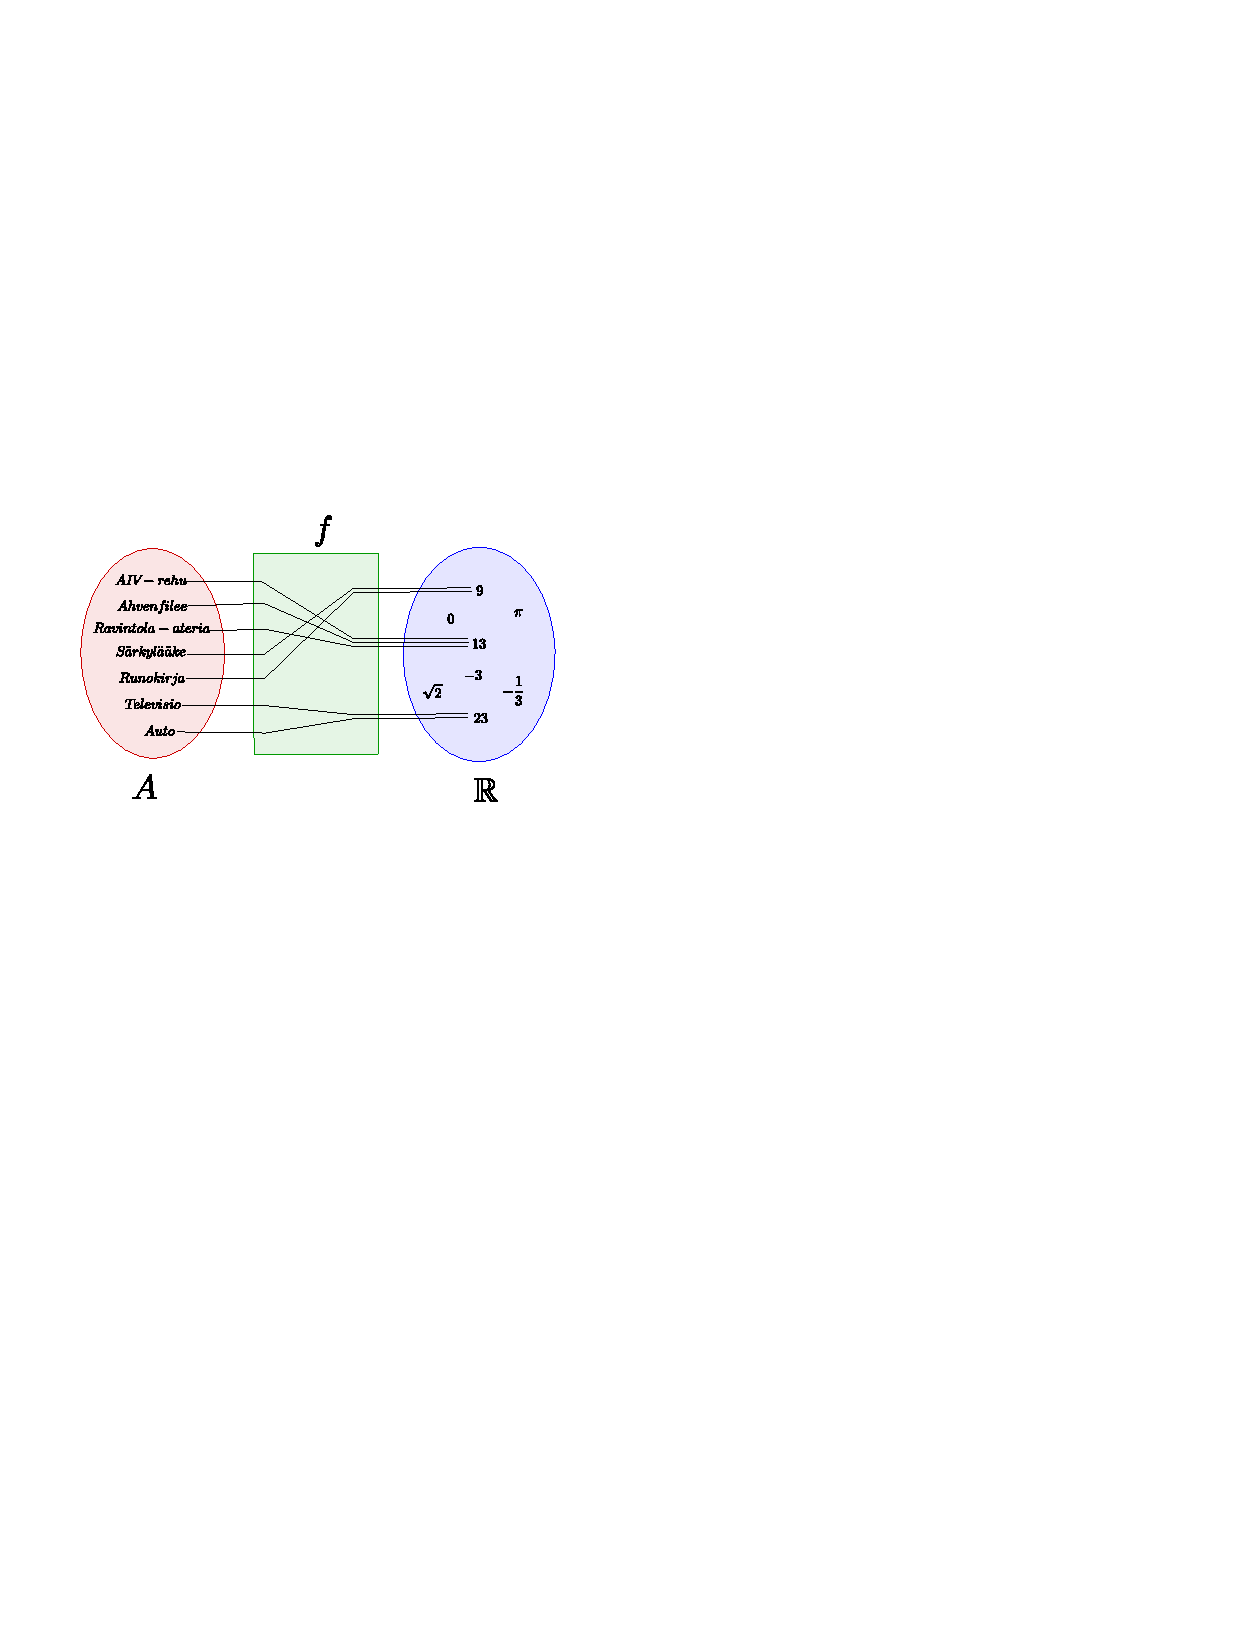
\includegraphics[width=13cm]{03-funktiot/kuvia/funktiokone.pdf}
\end{center}
\end{esimerkki}

Funktioiden käyttämiseen liittyy joitakin vakiintuneita tapoja:
\begin{itemize}
\item $f(x) = y$ lausutaan: ''Funktio saa arvon $y$ pisteessä $x$'',
\item Funktion määrittely- ja arvojoukko jätetään usein merkitsemättä, jos ne voidaan päätellä asiayhteydestä. Tällä kurssilla arvojoukkona on yleensä reaaliluvut.
\item Toisinaan funktiolle ja funktion kuvaajalle ei tehdä selkeää eroa:
$y = f(x)$ samaistetaan koordinaatistoon piirretyn funktion kuvaajan kanssa.
Periaatteessa funktio ja sen kuvaaja ovat kuitenkin eri asioita.
\end{itemize}

Funktiolla on usein jokin selkeä sääntö, joka voidaan kirjoittaa
matemaattisena lausekkeena.

\begin{esimerkki}
Jos neliön sivun pituutta merkitään $x$:llä, voidaan sivun pituuden
ja neliön pinta-alan välistä yhteyttä kuvata funktiolla
$A(x) = x^2$.
\end{esimerkki}

Funktion määrittelyjoukko koostuu niistä muuttujan arvoista, joilla
funktio on määritelty eli joilla funktion arvo voidaan laskea.

\begin{esimerkki}
Määritellään funktio $f$ lausekkeella
\[
f(x) = \frac{1}{x-1}.
\]
Mikä on funktion määrittelyjoukko?

\textbf{Ratkaisu.}
Funktio $f(x)$ on määritelty, kun nimittäjä $x-1$ on erisuuri
kuin 0. Tämä toteutuu kaikilla $x$:n arvoilla lukuun ottamatta
arvoa $x = 1$. Funktion määrittelyjoukkoon kuuluvat siis
kaikki reaaliluvut paitsi luku $1$.
\end{esimerkki}

Funktion \emph{arvojoukko} sisältää ne maalijoukon alkiot,
jotka funktio saa arvokseen ainakin yhdessä pisteessä.

\esimerkki{
Mikä on edellä määritellyn funktion $f(x)$ arvojoukko?

\textbf{Ratkaisu.}
Arvojoukon selvittämiseksi tutkitaan, millä luvun $a$ arvoilla
yhtälöllä $f(x) = a$ on ratkaisu,
\begin{align*}
a &= \frac{1}{x-1} & &| \, \text{Oletetaan, että $x \neq 1$, jolloin voimme kertoa $(x-1)$:llä puolittain.} \\
a(x-1) &= 1 \\
x-1 &= \frac{1}{a} \\
x &= 1+\frac{1}{a} & &| \, \text{Havaitaan, että yhtälöllä on ratkaisu
kaikilla $a \neq 0$.}
\end{align*}
Funktion arvojoukkona on siis koko reaalilukujen joukko poislukien luku $0$.
}


\section*{Tehtäviä}
\begin{tehtava}
Olkoon $f(x)=\frac{2^x+4}{x}$. Laske
\begin{enumerate}[a)]
\item $f(1)$
\item $f(2)$
\item $f(\frac{1}{2})$
\item $f(\frac{1}{3})$
\item $f(0)$
\item $f(-1)$
\end{enumerate}
\begin{vastaus}
\begin{enumerate}[a)]
\item $6$
\item $4$
\item $2\sqrt{2}+8$
\item $3\sqrt[3]{2}+12$
\item ei määritelty
\item $\frac{-9}{2}$
\end{enumerate}
\end{vastaus}
\end{tehtava}

% kai vaikeahko
\begin{tehtava}
Millä $x$:n arvoilla yhtälö $f(f(x)) = x$ pätee, kun
\begin{enumerate}[a)]
\item $f(x) = 1$
\item $f(x) = x$
\item $f(x) = x+1$
\item $f(x) = 2x$
\item $f(x) = 2x+1$?
\end{enumerate}

\begin{vastaus}
\begin{enumerate}[a)]
\item $x = 1$
\item kaikilla $x\in\mathbb{R}$
\item ei ratkaisuja
\item $x = 0$
\item $x = -1$
\end{enumerate}
\end{vastaus}
\end{tehtava}

    \chapter{Koordinaatisto ja funktion kuvaaja}
Funktioita reaaliluvuilta reaaliluvuille voidaan havainnollistaa koordinaatistossa kuvaajien avulla. Funktion $f$ kuvaajassa koordinaatistoon piirretään ne pisteet, joilla y-koordinaatti on $f$:n arvo sen x-koordinaatissa. Siis kaikilla $f$:n määrittelyjoukon luvuilla $x$ lasketaan $y = f(x)$ ja piirretään piste $(x, y)$ koordinaatistoon. Funktioita voi piirtää helposti myös graafisilla laskimilla tai tietokoneohjelmilla (esimerkiksi Wolfram Alphalla\footnote{\url{http://www.wolframalpha.com/}}).

% Tarvitaan kuvien ja taulukkojen vierekkäin laittamiseen.
\def\vcent#1{\mathsurround0pt$\vcenter{\hbox{#1}}$}

\begin{esimerkki}
Funktion $f(x) = \frac{x}{2} - 1$ kuvaaja sisältää kaikki pisteet $(x, y)$, joilla pätee $y = \frac{x}{2} - 1$:
\begin{center}
\begin{tabular}{cc}
\begin{tabular}{|r|l|}
\hline
$x$ & $y = f(x)$ \\
\hline
$-3$ & $-2,5$ \\
$-2$ & $-2$ \\
$-1$ & $-1,5$ \\
$0$ & $-1$ \\
$1$ & $-0,5$ \\
$2$ & $0$ \\
$3$ & $0,5$ \\
\hline
\end{tabular} &
\vcent{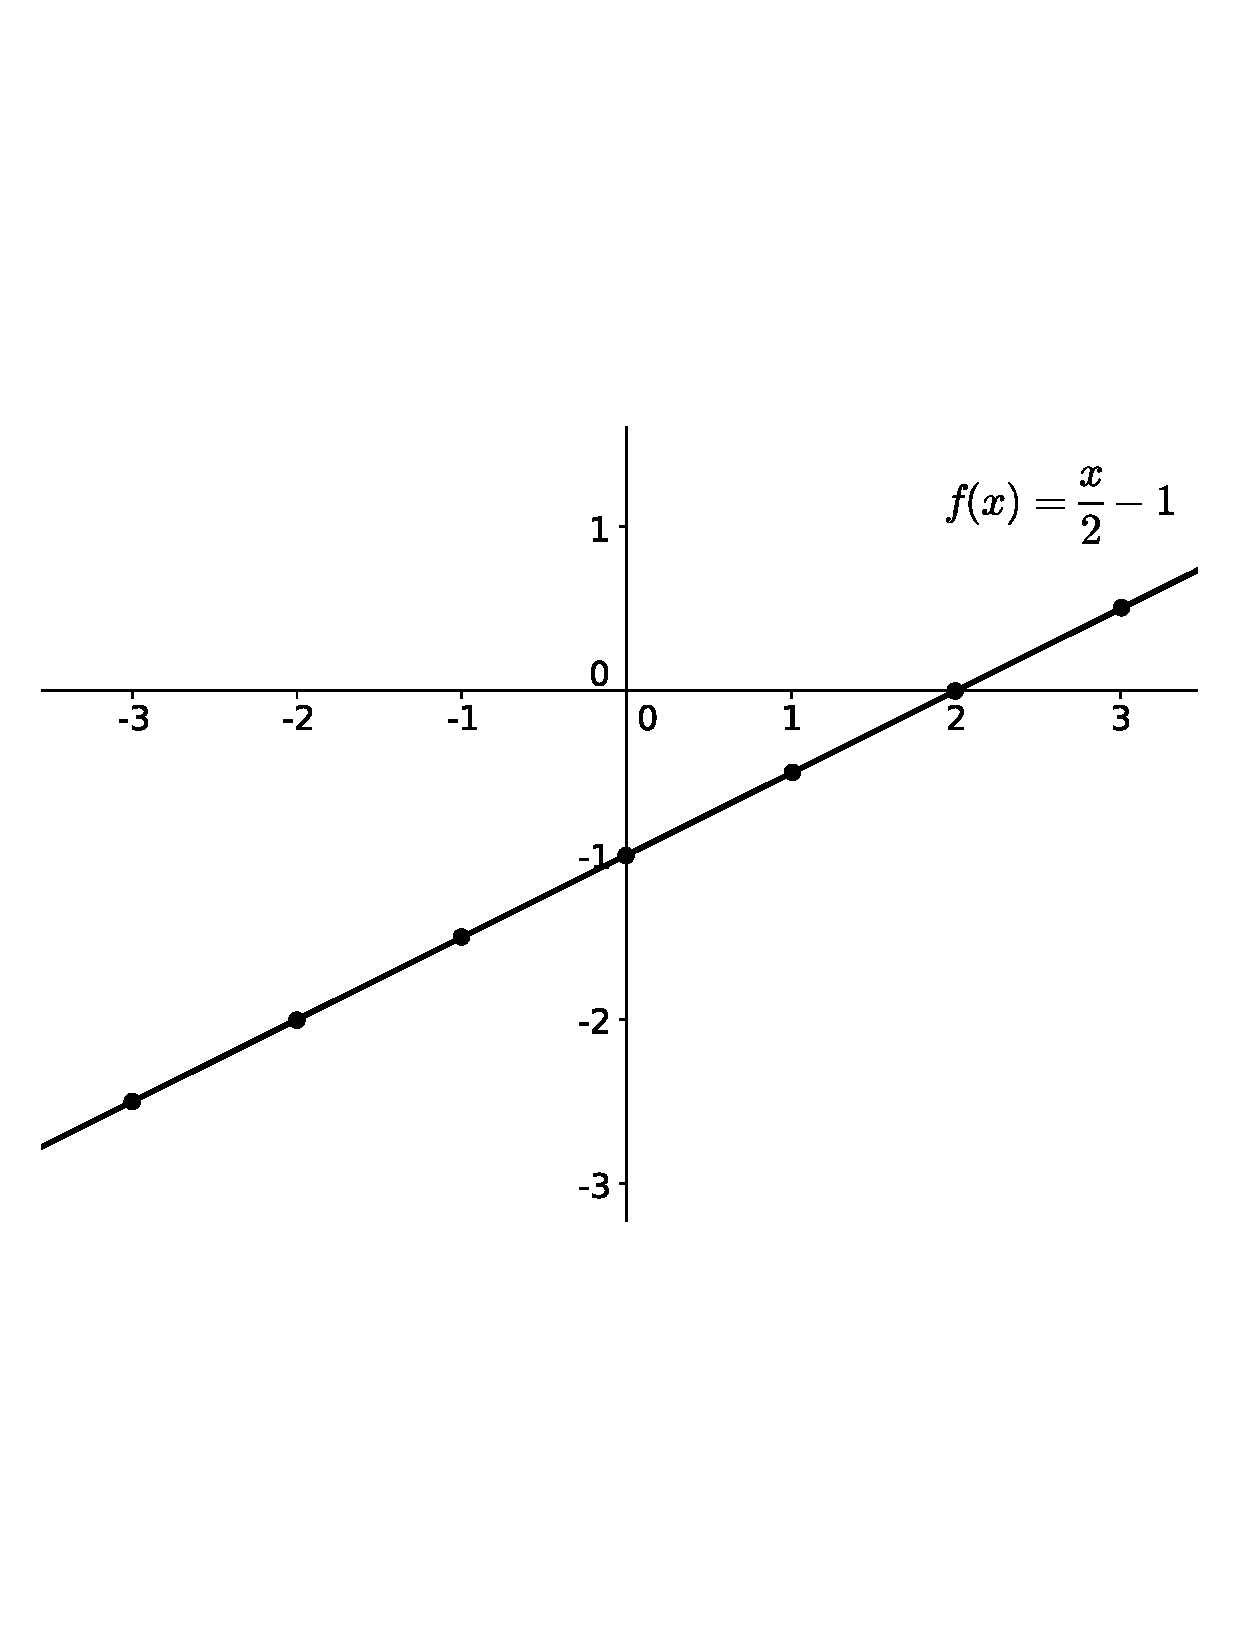
\includegraphics[width=8cm]{03-funktiot/kuvia/suoraesim.pdf}}
\end{tabular}
\end{center}
\end{esimerkki}

\begin{esimerkki}
Funktion $f(x) = x^2$ kuvaaja sisältää kaikki pisteet $(x, y)$, joilla pätee $y = x^2$:
\begin{center}
\begin{tabular}{cc}
\begin{tabular}{|r|l|}
\hline
$x$ & $y = f(x)$ \\
\hline
$-2$ & $4$ \\
$-1$ & $1$ \\
$-0,5$ & $0.25$ \\
$0$ & $0$ \\
$0,5$ & $0.25$ \\
$1$ & $1$ \\
$2$ & $4$ \\
\hline
\end{tabular} &
\vcent{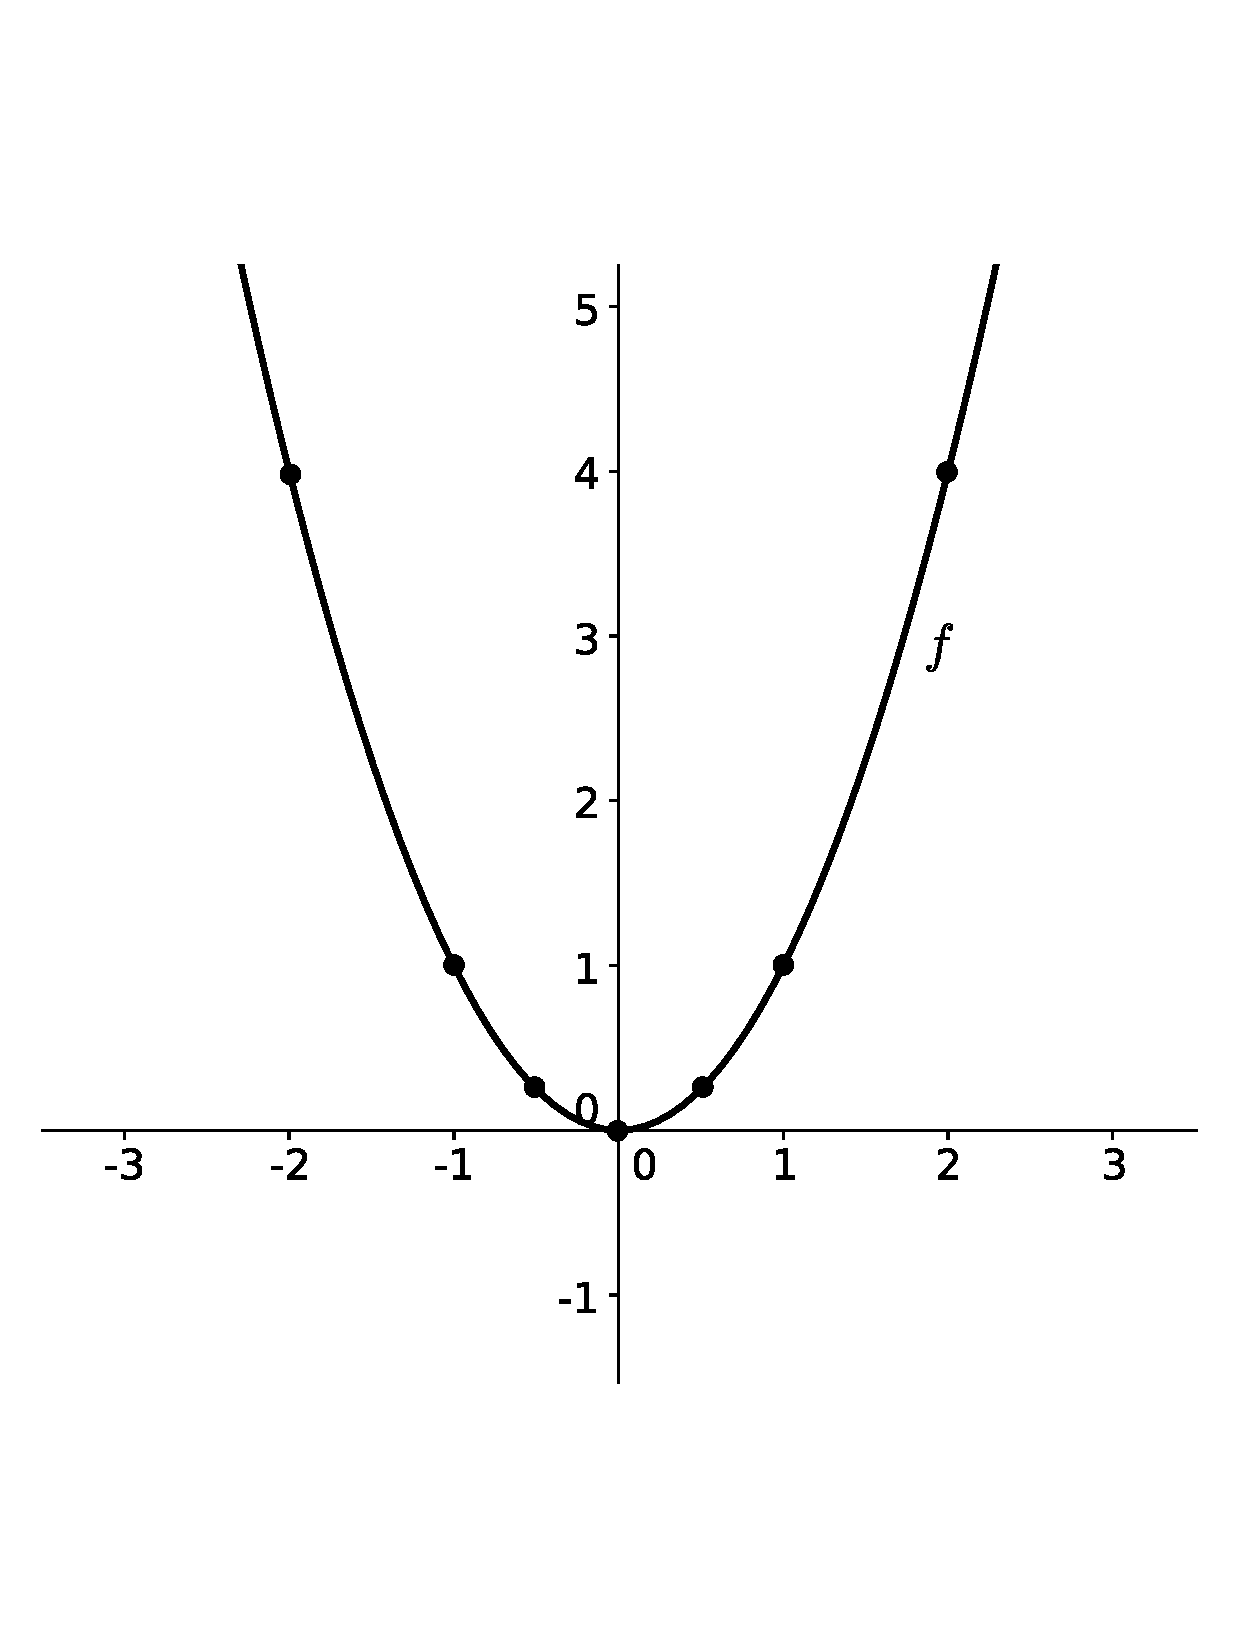
\includegraphics[width=6cm]{03-funktiot/kuvia/paraabeli.pdf}}
\end{tabular}
\end{center}
\end{esimerkki}

\begin{esimerkki}
Funktion $f(x) = x^3-5x+2$ kuvaaja sisältää kaikki pisteet $(x, y)$, joilla pätee $y = x^3-5x+2$:
\begin{center}
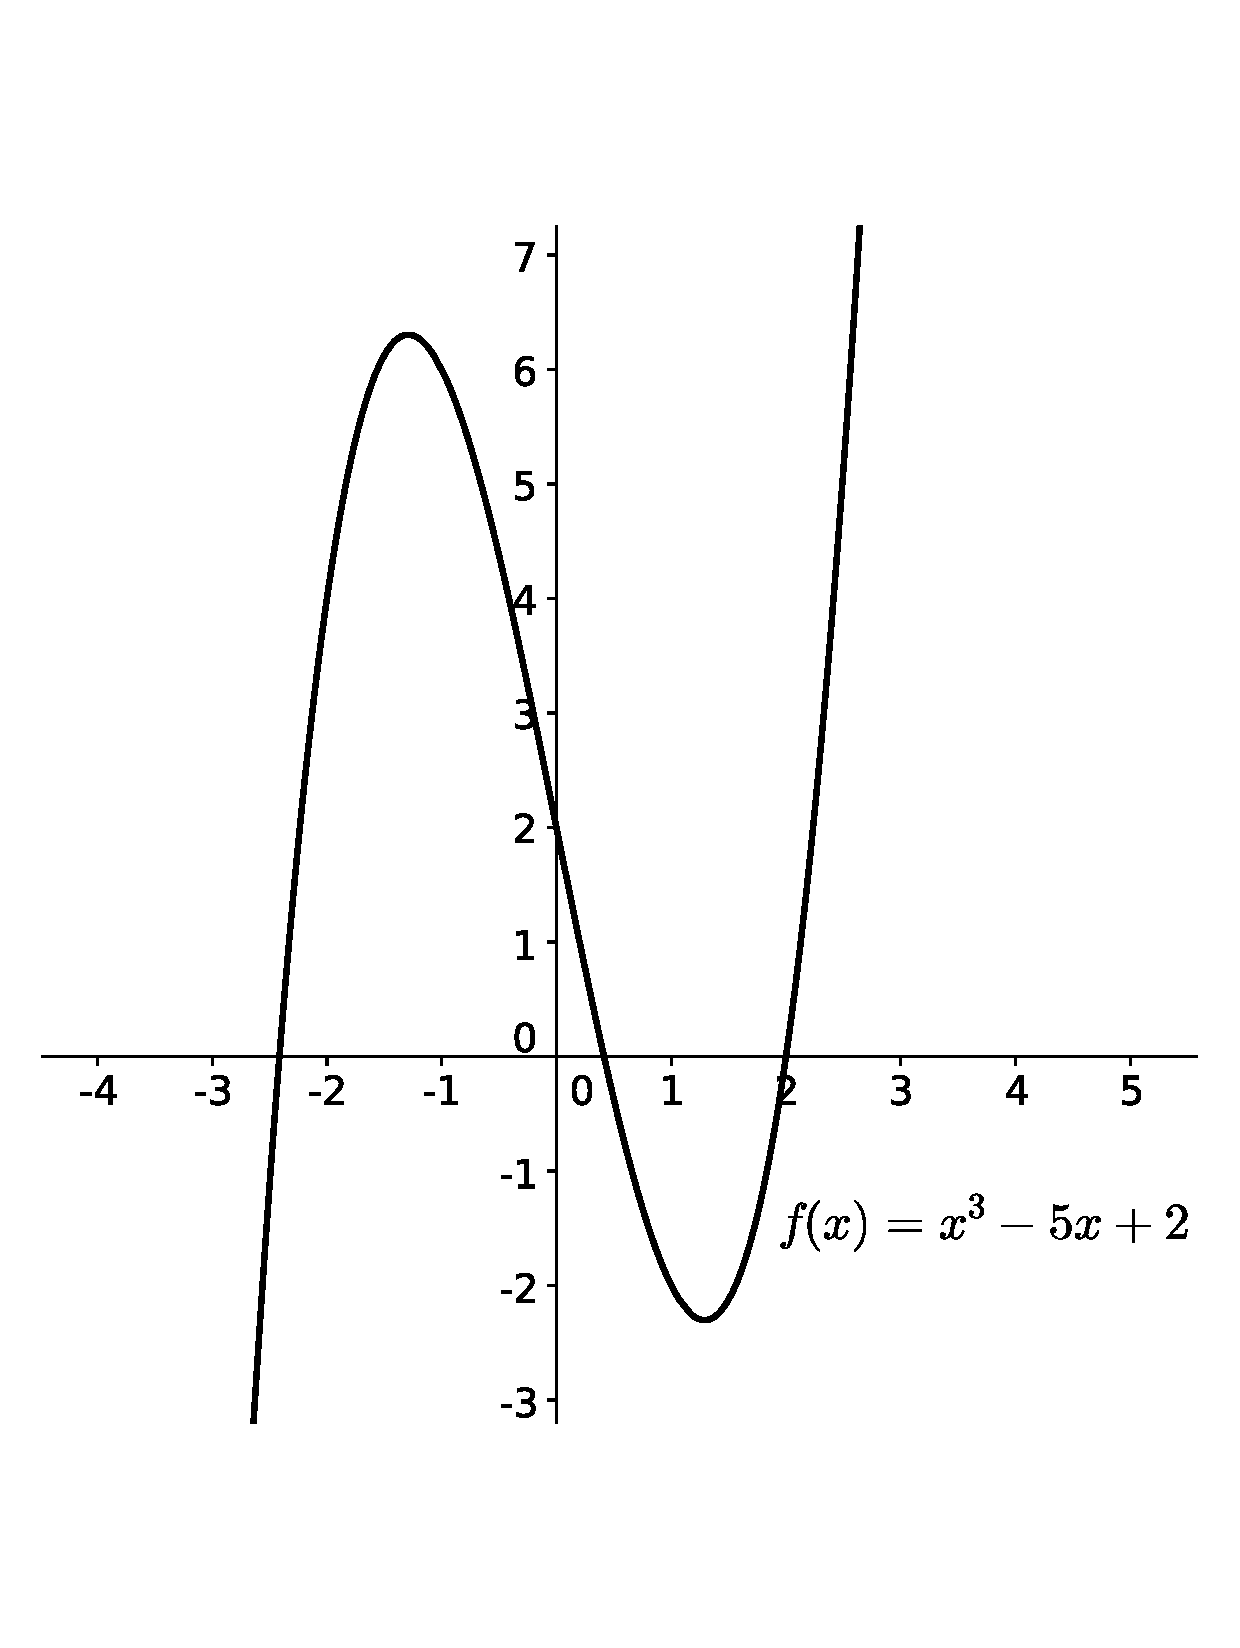
\includegraphics[width=7cm]{03-funktiot/kuvia/deg3polynomiesim.pdf}
\end{center}
\end{esimerkki}

\section*{Tehtäviä}

\subsubsection*{Opi perusteet}

\begin{tehtava}
Hahmottele funktion kuvaaja kynällä ja paperilla tai laskimen avulla. Voit myös käyttää tietokonetta.
\begin{enumerate}[a)]
\item $f(x) = 2$
\item $f(x) = 3x+2$
\item $f(x) = x^2$
\item $f(x) = \frac{2}{x}$
\end{enumerate}

%\begin{vastaus}
%\end{vastaus}
\end{tehtava}

    \chapter{Potenssifunktio}

Usein kahden muuttujan välinen riippuvuus ei ole selvästi suoraan
tai kääntäen verrannollista. Potenssifunktion käyttäminen on eräs
keino yrittää kuvata tällaisia riippuvuuksia.

\laatikko{Potenssifunktio on määritelty
$ f(x) = a x^n $, jossa $a \neq 0$. }

Eksponenttia $n$ kutsutaan potenssifunktion \emph{asteeksi}. Periaatteessa
potenssifunktion eksponentti voi olla mikä tahansa reaaliluku, mutta
rajoitumme ensin käsittelemään tapauksia, jossa $n = 1, 2, 3\ldots $.

\begin{esimerkki}
Jos neliön sivun pituus on $x$, neliön pinta-ala voidaan laskea
funktiolla $A(x)=x^2$.
Esimerkiksi jos $x = 3$ cm, saadaan neliön pinta-alaksi $A(x) = 9$ cm$^2$.
Vastaavasti kuutiolle: jos $x$ kuvaa kuution särmän pituutta, funktiolla
$V(x)=x^3$ voidaan laskea kuution tilavuus. Sekä $A(x)$ että $V(x)$ ovat
esimerkkejä potenssifunktioista.
\end{esimerkki}

Potenssifunktion aste vaikuttaa funktion kuvaajan muotoon:
\begin{itemize}
  \item
Jos aste on parillinen, kuvaaja on U-kirjaimen muotoinen ja funktio
saa $a$:n merkistä riippuen joko pelkästään positiivisia tai pelkästään
negatiivisia arvoja.
  \item
Jos aste on pariton, kuvaaja muodostaa ``kaksoismutkan'' ja potenssifunktio
saa sekä positiivisia että negatiivisia arvoja.
\end{itemize}

\missingfigure{Potenssifunktioiden kuvaajat - yksi parillisilla potensseilla ja toinen parittomilla (kerroin a positiivinen).}

Tärkeitä erikoistapauksia potenssifunktioista saadaan, kun asetetaan $n = 1$ tai
$n = -1$. Kun $n = 1$, saadaan edellisessä luvussa esitelty suoraan verrannollinen
riippuvuus $x$:n ja $f(x)$:n välillä, ja kun $n = -1$, muuttuja $x$ ja
funktion arvo $f(x)$ ovat kääntäen verrannolliset.

Potenssifunktiota voidaan laajentaa niin, että sallitaan eksponentille $n$
myös negatiiviset arvot.
Tällöin funktion muoto muuttuu merkittävästi. Funktio ei myöskään ole
enää määritelty, kun $x = 0$, vaan funktion arvot näyttävät
``räjähtävän äärettömyyteen'', kun y-akselia lähestytään:

\missingfigure{Potenssifunktioiden kuvaajat - yksi potenssilla -1
ja toinen potenssilla -2.}

%Potenssifunktiota käsitellään samalla lailla riippumatta eksponentin
%etumerkistä. Huomaa kuitenkin, että $\frac{1}{x^n} \neq 0 $ kaikilla $x$:n %arvoilla.

%Tästä alaspäin on potenssiyhtälöitä, jotka varmaan menee jo päälle
%aiemmin käydyn asian kanssa. Sekaannus meikäläisen osalta... -Matti


    \chapter{Eksponenttifunktio}

Potenssifunktiossa $f(x) = x^n$ muuttuja $x$ on kantalukuna. Jos muuttuja
$x$ on sen sijaan eksponenttina, saadaan joukko funktioita, joita
kutsutaan \emph{eksponenttifunktioiksi}.

\laatikko{Eksponenttifunktiot ovat muotoa $f(x) = a^x$, $a > 0$,
$a \neq 1$ olevia funktioita.}

Eksponenttifunktioita on kahta tyyppiä: kasvavia ja väheneviä.
Kasvavilla eksponenttifunktioilla $a>1$, esimerkiksi

\begin{center}
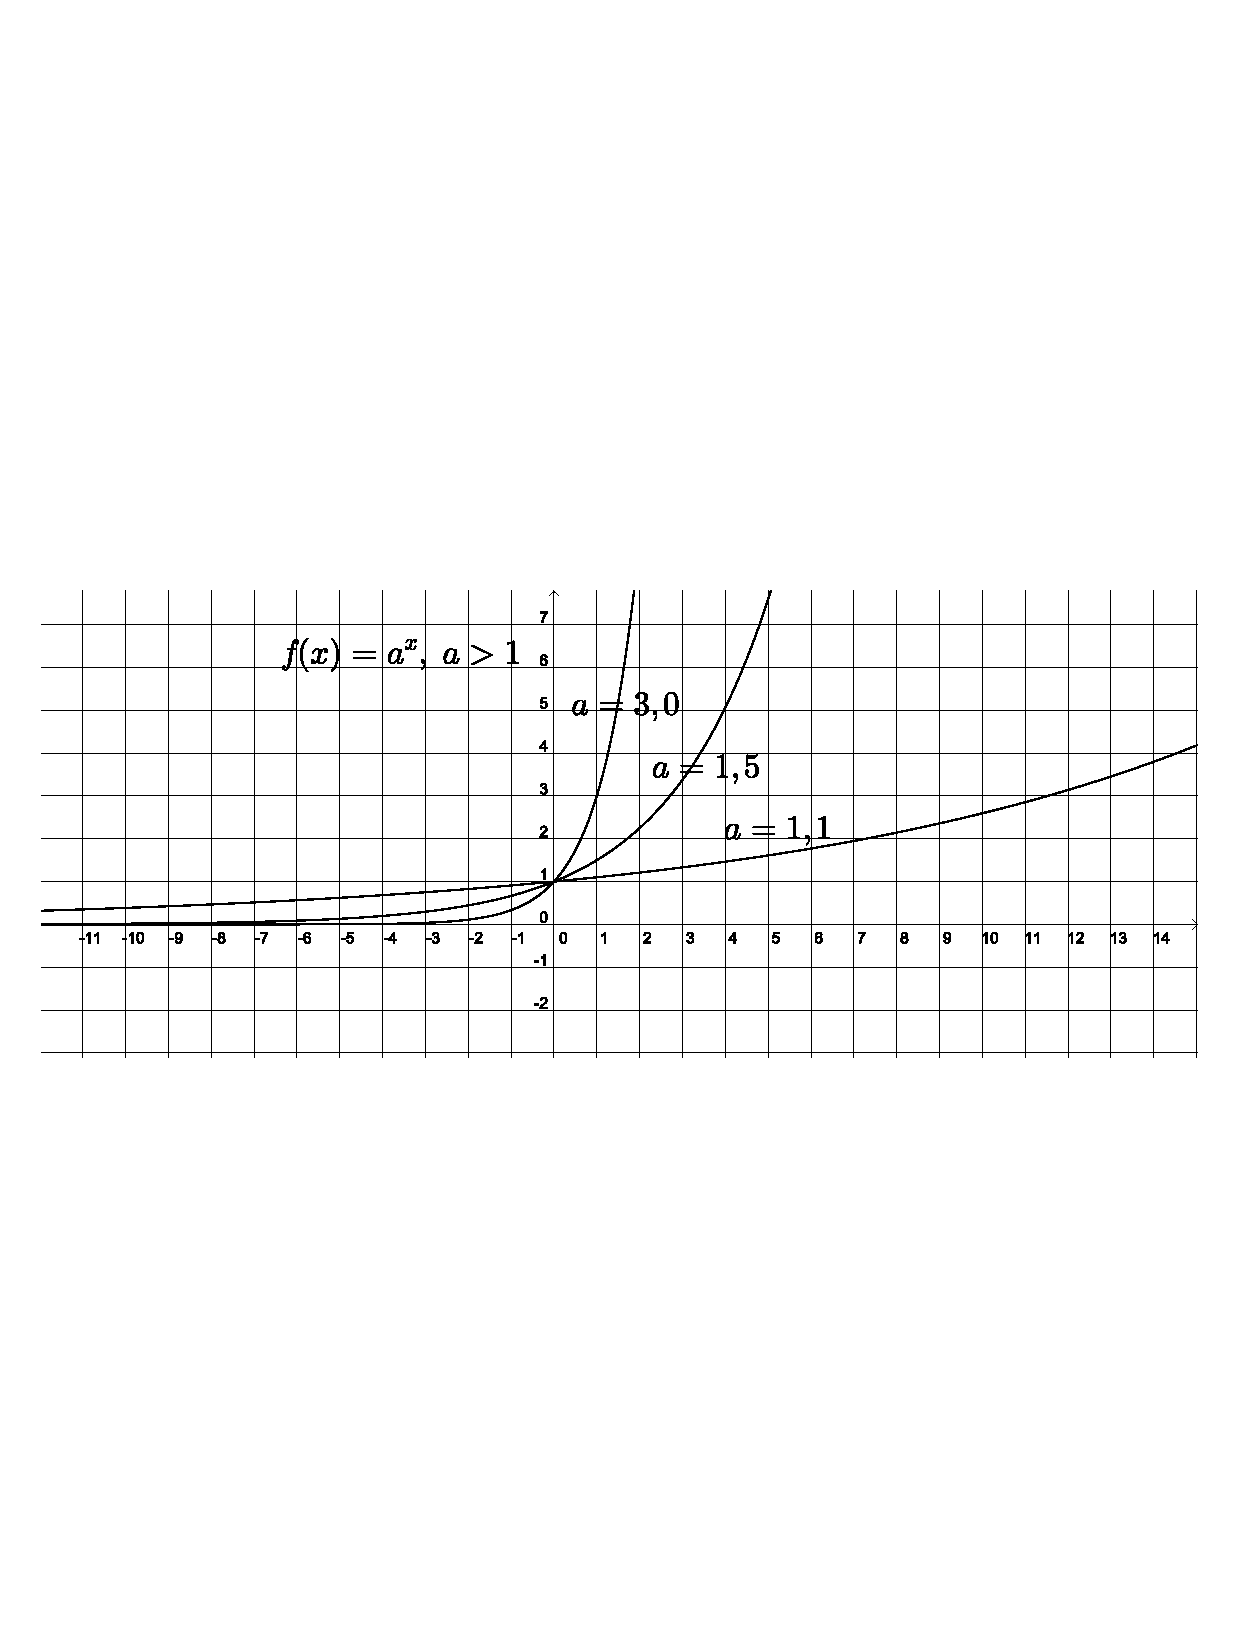
\includegraphics{03-funktiot/kuvia/apotenssiinxaisompikuinyksi.pdf}
\end{center}

Vähenevillä eksponenttifunktioilla $0<a<1$, esimerkiksi

\begin{center}
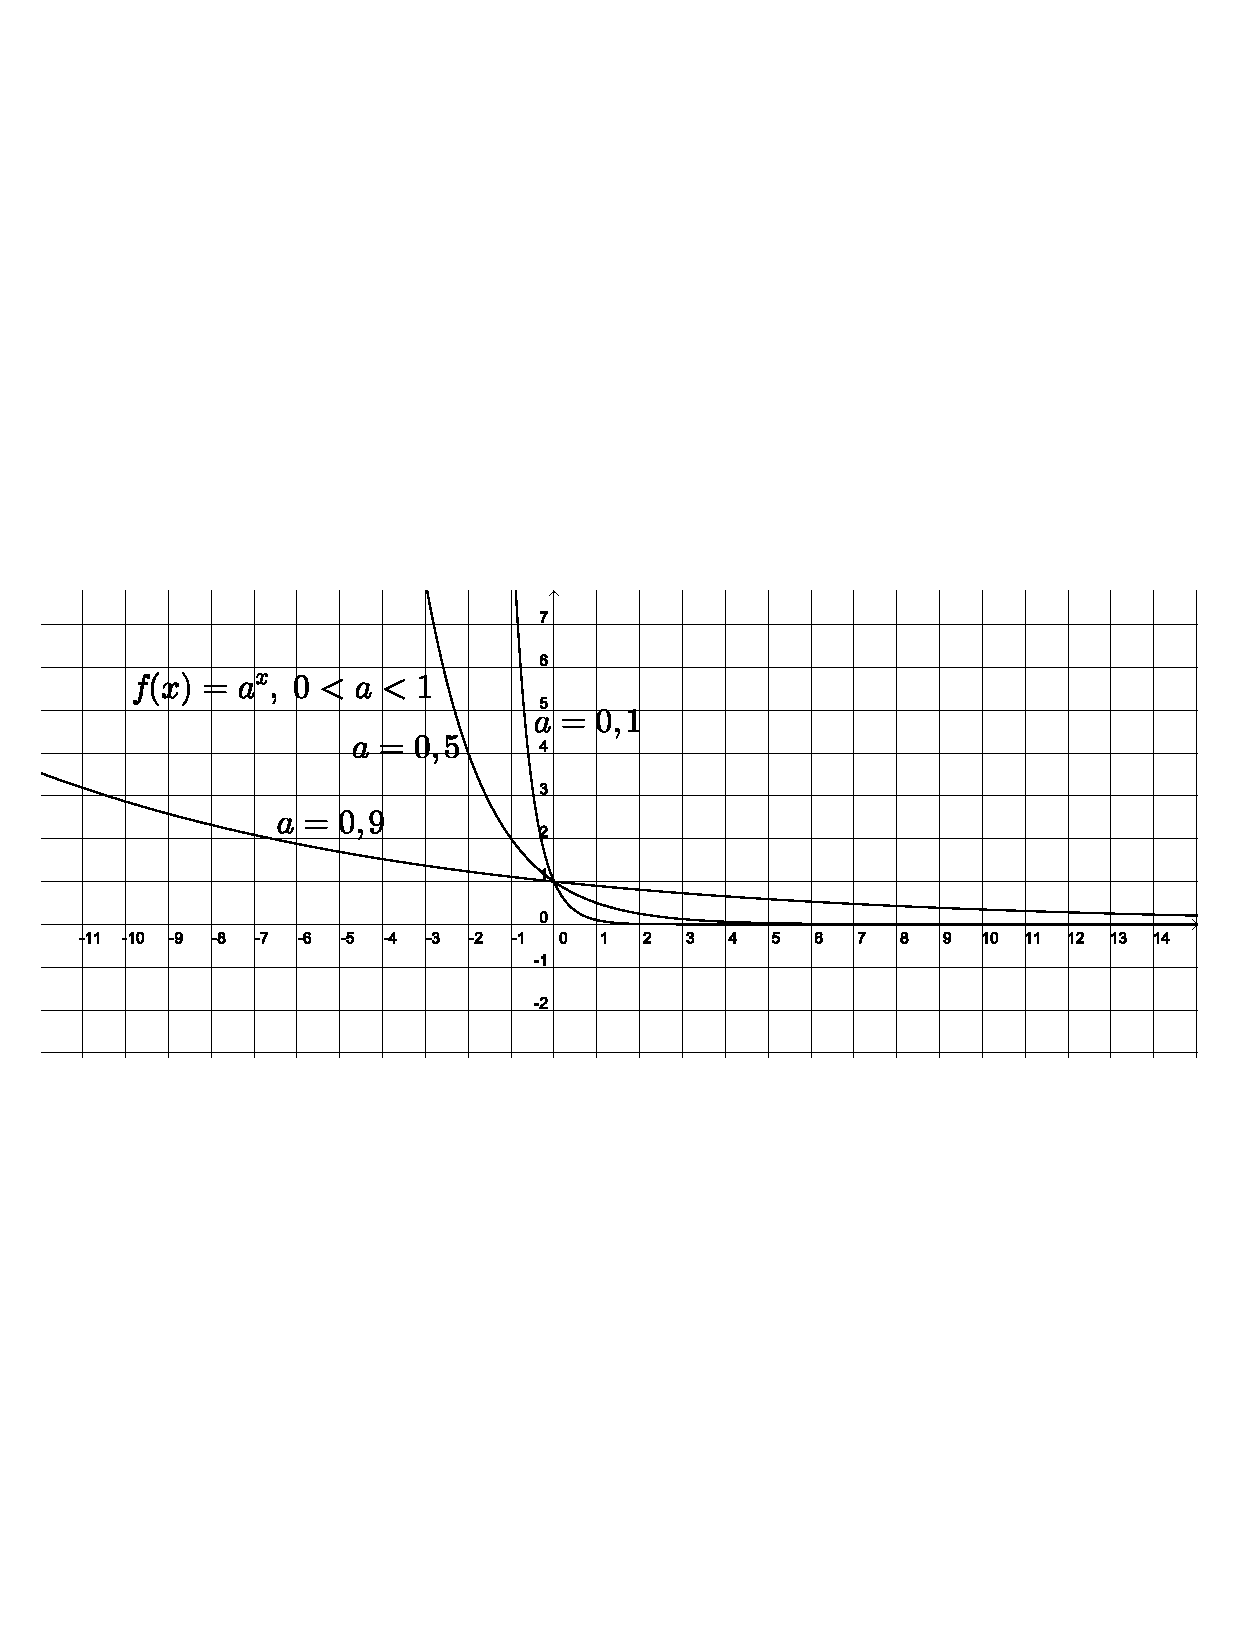
\includegraphics{03-funktiot/kuvia/apotenssiinxaisompikuinnolla.pdf}
\end{center}

Negatiiviselle kantaluvulle ei ole määritelty yleistä reaalilukupotenssia, 
joten eksponenttifunktiota ei ole määritelty, kun $a < 0$. 

Kun $a=0$ tai $a=1$, eksponenttifunktio pelkistyy vakiofunktioksi.
Lisäksi $0^0$:a ei ole määritelty, joten vaaditaan, että
eksponenttifunktion kantaluvulle $a$ pätee $a>0$ ja $a \neq 1$.

%\emph{Eksponenttiyhtälö} muodostuu, kun kysytään, millä $x$:n arvoilla %eksponenttifunktio saavuttaa tietyn arvon.

\begin{esimerkki}
Millä muuttujan $x$ arvoilla eksponenttifunktio $f(x) = 2^x$ saa arvon
$f(x) = 64$?

\textbf{Ratkaisu.}
Kirjoitetaan tehtävä yhtälöksi: $2^x = 64$. Kokeilemalla huomataan,
että $x = 6$ ratkaisee yhtälön.

Varmistutaan vielä siitä, että yhtälöllä ei ole muita ratkaisuja.
Eksponenttifunktion kantalukuna on $2$, joten eksponenttifunktio on
kasvava. Funktio $f(x) = 2^x$ ei siis voi saada uudelleen arvoa $64$,
kun $x > 6$. Samasta syystä $f(x)$ ei voi olla $64$, kun $x < 6$.

Ainoa ratkaisu yhtälölle on siis $x = 6$.
\end{esimerkki}

\begin{esimerkki}
Millä muuttujan $x$ arvoilla eksponenttifunktio
$f(x) = \left( \frac{1}{2} \right)^{x}$ saa arvon
$f(x) = 1/5$?

\textbf{Ratkaisu.}
Edellisen esimerkin tavoin kokeillaan $x$:n eri arvoja. Havaitaan,
että kun $x = 2$, funktio saa arvon $f(x) = \frac{1}{4}$, ja
kun $x = 3$, on $f(x) = \frac{1}{8}$. Ratkaisu on siis välillä
$2 < x < 3$.

Ratkaisun etsimistä voidaan jatkaa kokeilemalla esimerkiksi
arvoa $x = 2,5$. Näin päästään lähemmäksi ratkaisua, mutta
yhtälön ratkaisu on irrationaalinen, joten sen desimaalikehitelmä
on äärettömän pitkä ja jaksoton. Tarkkaa ratkaisua ei siis saada tällä menetelmällä.

Yleisen eksponenttiyhtälön tarkkaan ratkaisemiseen palataan myöhemmillä
matematiikan kursseilla.
\end{esimerkki}


\section{Eksponentiaalinen malli}

Kun eksponenttifunktiota käytetään kuvaamaan jotakin reaalimaailman
ilmiötä, siitä käytetään nimeä \emph{eksponentiaalinen malli}.

Eksponentiaalinen malli on eräs yleisimmin käytetyistä matemaattisista
malleista. Sillä kuvataan sellaista kasvua tai vähenemistä, jossa
kullakin ajanhetkellä funktion hetkellinen muutos on suoraan
verrannollinen funktion sen hetkiseen arvoon. Tämä muotoillaan
täsmällisesti myöhemmillä matematiikan kursseilla.

\begin{esimerkki}
Soluviljelmässä olevien \emph{Escherichia coli} -bakteerien
määrää voidaan kuvata eksponentiaalisella mallilla: ajanhetkellä
$t = 0$ bakteerien lukumäärä on $1$, ja kullakin aika-askeleella
bakteerien lukumäärä tuplaantuu. Malli voidaan kirjoittaa
\[
f(t) = 2^t, t \ge 0,
\]
jossa $f(t)$ on bakteerien lukumäärä ajanhetkellä $t$.
\sivulaatikko{
Huomaa, että esimerkissä funktion $f(t)$ arvot voivat
olla myös rationaalisia tai irrationaalisia, vaikka bakteerien
määrä on kokonaisluku. Yleensä tätä ei pidetä ongelmallisena,
vaan funktiota voidaan käsitellä, ikään kuin bakteerien määrä
olisi jatkuvasti kasvava suure.
}
\end{esimerkki}

\begin{esimerkki}
Radioaktiivisessa hajoamisessa atomiydinten lukumäärää kuvataan
eksponentiaalisella mallilla. Jos ydinten määrä ajanhetkellä
$t = 0$ on $f(t) = k$, malli voidaan kirjoittaa
\[
f(t) = k \cdot \left( \frac{1}{2} \right)^t, t \ge 0,
\]
jossa $f(t)$ on atomiydinten lukumäärä ajanhetkellä $t$. Atomiydinten
lukumäärä siis puolittuu kullakin aika-askeleella.
\end{esimerkki}

\section*{Tehtäviä}

\subsubsection*{Opi perusteet}

\begin{tehtava}
Olkoon $f(x) = 4^x$. Laske
\begin{enumerate}[a)]
\item $f(0)$
\item $f(3)$
\item $f(\frac{1}{2})$
\end{enumerate}
\begin{vastaus}
\begin{enumerate}[a)]
\item $1$
\item $64$
\item $2$
\end{enumerate}
\end{vastaus}
\end{tehtava}

\begin{tehtava}
Olkoon $f(x) = 10^x$. Millä $x$:n arvoilla
\begin{enumerate}[a)]
\item $f(x) = 1000$
\item $f(x) = \frac{1}{100}$
\item $f(x) = -1$?
\end{enumerate}
\begin{vastaus}
\begin{enumerate}[a)]
\item $3$
\item $6$
\item Ei ratkaisua.
\end{enumerate}
\end{vastaus}
\end{tehtava}

\subsubsection*{Hallitse kokonaisuus}
\begin{tehtava}
Minkä kahden kokonaisluvun välissä yhtälön
$10^x = 500$ ratkaisu on?
\begin{vastaus}
Ratkaisu on lukujen $2$ ja $3$ välissä.
\end{vastaus}
\end{tehtava}


\begin{tehtava}
Olkoon $f(t) = 20 \cdot 2^t$ bakteerien lukumäärä soluviljelmässä
ajanhetkellä $t$. Millä ajanhetkellä bakteerien lukumäärä on tasan 160?
\begin{vastaus}
Ajanhetkellä $t = 3$.
\end{vastaus}
\end{tehtava}

\begin{tehtava}
Miten muokkaisit edellisen tehtävän funktiota, jos bakteerien lukumääräksi
halutaan 5 ajanhetkellä $t = 0$?
\begin{vastaus}
$f(t) = 5 \cdot 2^t$
\end{vastaus}
\end{tehtava}

\begin{tehtava}
Millä ajanhetkellä atomiydinten määrä on alle $1/200$ alkuperäisestä?
\begin{vastaus}
Ajanhetkellä $t = 8$.
\end{vastaus}
\end{tehtava}

\subsubsection*{Sekalaisia tehtäviä}

\begin{tehtava}
(YO 1877 4) Vuosikymmenen 1860--70 kuluessa lisääntyi Helsingin väkiluku puolella vuoden 1860 väkiluvulla. Jos väkiluvun lisäys tapahtuisi seuraavinakin vuosikymmeninä samassa suhteessa, paljonko väkeä Helsingissä olisi 1890, kun siellä 1860 oli 21~700 asukasta? 
	\begin{vastaus}
	73~200 (pyöristämättä 73~237,5)
	\end{vastaus}
\end{tehtava}


% % tähän parempi tehtävä atomiytimistä
%\begin{tehtava}
%Millä ajanhetkellä atomiydinten määrä on alle $1/200$ alkuperäisestä?
%\begin{vastaus}
%Ajanhetkellä $t = 8$.
%\end{vastaus}
%\end{tehtava}

    % Osan "Funktiot" kertaus.
\chapter{Kertaus}


\part{Kertaustehtäviä}
    \input{05-loppuosa/02-yo-tehtavia}
    \chapter{''Näihin pystyt jo'' -pääsykoetehtäviä}

\section{Arkkitehtuuri}

\section{Fysiikka}

\section{Kansantaloustiede}

\section{Kauppatieteellinen}

\section{Tekniikan ala (AMK)}

\section{Tekniikan ala (diplomi-insinööri)}
\begin{description}
	\item[(2012/3)] Asumistukea maksetaan 80 \% vuokran määrästä, siltä osin kuin vuokra ei ylitä 252 euroa. Vuokran määrää vähennettynä asumistuella kutsutaan omavastuuksi.
		\begin{enumerate}[(a)]
			\item Minka suuruinen vuokra on, kun omavastuu on puolet vuokrasta?
		\end{enumerate}
	
	\item[(2009/1)] Kokonaistuotanto jaetaan materian ja palveluiden tuotantoon. Verrataan tuotantoa tammikuussa 2008 tammikuuhun 2009. Tänä vuoden pituisen tarkastelujakson aikana materiatuotanto kasvoi 2,0 \% ja palvelutuotanto laski 7,0 \%.
	
	Kuinka suuri oli materiatuotannon osuus kokonaistuotannosta tammikuussa 2009,
	\begin{enumerate}[(a)]
		\item kun tammikuussa 2008 materia- ja palvelutuotanto olivat yhtäsuuret?
		\item kun vertailuaikana kokonaistuotanto laski 2,0 \%?
	\end{enumerate}
	Anna kummatkin vastaukset 0,1 \%-yksikön tarkkuuteen pyöristettynä.

	\item[(2008/2)] Yritys hankkii 5000 kg raaka-ainetta, josta on vettä 5,40 \% (painoprosenttia) ja väripigmenttiä 2,60 \%. Ennen käyttöä raaka-aine on laimennettava siten, että lisäyksen jälkeen sekoituksesta 6,60 \% on vettä.
	
	\begin{enumerate}[(a)]
		\item Miten paljon hankittuun raaka-aineeseen tulee lisätä vettä, jotta haluttu vesipitoisuus saavutetaan?
		\item Miten paljon vettä ja väripigmenttiä tulee lisätä hankittuun raaka-aineeseen, jotta haluttu vesipitoisuus saavutetaan, ja lisäksi väripigmentin suhteellinen osuus massasta säilyy alkuperäisenä 2,60 \%:na?
	\end{enumerate}
	Anna vastaukset sadan gramman tarkkuudella.

	\item[(2007/1)] Vaaleissa kaikkiaan 39 300 äänestäjästä 45 \% äänestää varmasti puoluetta A ja 47 \% puoluetta B. Loput ovat ns. liikkuvia äänestäjiä, jotka eivät ole vielä päättäneet kantaansa.
	
	\begin{enumerate}[(a)]
		\item Oletetaan, että kaikki äänioikeutetut äänestävät. Kuinka monta liikkuvien äänestäjien ääntä puolueen A täytyy tällöin kerätä saadakseen enemmistön, vähintään puolet annetuista äänistä?
		\item Oletetaan, että täsmälleen kolmasosa liikkuvista äänestäjistä jättää äänestämättä. Kuinka monta prosenttia liikkuvien äänestäjien annetuista äänistä puolueen A täytyy tällöin kerätä saadakseen enemmistön kaikista annetuista äänistä?
	\end{enumerate}	 	
	
\end{description}


\section{Tilastotiede}




\part{Liitteet}
    \chapter{Lähtötasotesti}

(Tää tulee oikeasti ennen tätä chapteria ja osaa)

\begin{tehtava}
\begin{enumerate}
\item Laske $2^2+2 \cdot 2+2$
\item sasdas
\item 
\end{enumerate}

\begin{vastaus}
\begin{enumerate}
\item 
\item
\item

\end{enumerate}
\end{vastaus}
\end{tehtava}

    \chapter{Suureista ja yksiköistä}

\laatikko{
Kerrannaisyksiköiden etuliitteet:

\begin{tabular}{c|c}
\begin{tabular}{c|c|c}
Nimi & Kerroin & Tunnus \\
\hline
deka & $10^{1}$ & da 	\\
hehto & $10^{2}$ & h 	\\
kilo & $10^{3}$ & k 	\\
mega & $10^{6}$ & M 	\\
giga & $10^{9}$ & G		\\
tera & $10^{12}$ & T 	
\end{tabular}
\begin{tabular}{c|c|c}
Nimi & Kerroin & Tunnus \\
\hline
desi & $10^{-1}$ & d 	\\
sentti & $10^{-2}$ & c 	\\
milli & $10^{-3}$ & m	\\
mikro & $10^{-6}$ & mu \\
nano & $10^{-9}$ & n 	\\
piko & $10^{-12}$ & p
\end{tabular}
\end{tabular}
}

\laatikko{
Yksi tunti on $60$ minuuttia. Yksi minuutti on $60$ sekuntia.
\begin{equation}
1 \text{h} = 60 \text{min}
\end{equation}
\begin{equation}
1 \text{min} = 60 \text{s}
\end{equation}
\begin{equation}
1 \text{h} = 60 \text{min} = 60 \cdot 60 \text{s}
\end{equation}
}

\begin{esimerkki}
Kuinka monta minuuttia on $1,25$ h? $1,25 \text{h} = 1,25 \cdot 60 \text{min} = 75 \text{min}$. $1,35$ h on siis $75$ minuuttia. Huomaa, että voit laskuissasi esittää desimaaliluvun $1,25$ yhdistettynä lukuna $1 \frac{25}{100}$ eli $1 \frac{1}{4}$, mikä saattaa helpottaa laskemista.
\end{esimerkki}

\todo{pitää täydentää esittelyä kerrannaisyksiköistä ( mitä on mega, milli, sentti jne)}
\todo{kuinka monta metriä on tuuma jne. (riittänee mainita tehtäviin?)}
\todo{merkitsevät numerot}

Tietotekniikassa datan määrää mitataan tavuina, mutta siellä yksi kilotavu (kt) ei tarkoita tasan 1000 tavua,  vaan 1024 tavua ($2^10$). Vastaavasti yksi megatavu on 1024 kt eli ($1048576 = 2^20$ tavua) , yksi gigatavu 1024 Gt jne.

\begin{tehtava}
Muuta minuuteiksi
\begin{enumerate}
\item $1$ h $17$ min
\item $2$ h $45$ min
\item $1,5$ h
\item $1,75$ h
\end{enumerate}
\begin{vastaus}
\begin{enumerate}
\item $77$ min
\item $165$ min
\item $90$ min
\item $105$ min
\end{enumerate}
\end{vastaus}
\end{tehtava}

\begin{tehtava}
Muuta sekunneiksi
\begin{enumerate}
\item $1$ h $42$ min
\item $3$ h $32$ min
\item $1,25$ h
\item $4,5$ h
\end{enumerate}
\begin{vastaus}
\begin{enumerate}
\item $6120$ s
\item $12720$ s
\item $4500$ s
\item $16200$ s
\end{enumerate}
\end{vastaus}
\end{tehtava}

\begin{tehtava}
Muuta tunneiksi ja minuuteiksi
\begin{enumerate}
\item $125$ min
\item $667$ min
\item $120$ min
\item $194$ min
\end{enumerate}
\begin{vastaus}
\begin{enumerate}
\item $2$ h $5$ min
\item $11$ h $7$ min
\item $2$ h
\item $3$ h $14$ min
\end{enumerate}
\end{vastaus}
\end{tehtava}


\begin{tehtava}
Esitä luku ilman kymmenpotenssia.
\begin{enumerate}
\item $3,2 \cdot 10^4$
\item $-7,03 \cdot 10^{-5}$
\item $10,005 \cdot 10^{-2}$
\end{enumerate}
\begin{vastaus}
\begin{enumerate}
\item $32000$
\item $-0,0000703$
\item $0,10005$
\end{enumerate}
\end{vastaus}
\end{tehtava}

\begin{tehtava}
Esitä luku ilman etuliitettä.
\begin{enumerate}
\item $0,5$ dl
\item $233$ mm
\item $33$ cm
\item $16$ kg
\item $2$ MJ
\item $4$ kt
\item $0,125$ Mt
\end{enumerate}
\begin{vastaus}
\begin{enumerate}
\item $0,05$ l
\item $0,233$ m
\item $0,33$ m
\item $16 000$ g
\item $2 000 000$ J
\item $4096$ tavua
\item $131072$ tavua
\end{enumerate}
\end{vastaus}
\end{tehtava}

\begin{tehtava}
Muuta seuraavat pituudet SI-muotoon (1 tuuma = 2,54 cm, 1 jaardi = 0,914 m, 1 jalka = 0,305 m, 1 maili = 1,609 km).
\begin{enumerate}
\item 5 tuumaa senttimetreiksi
\item 0,3 tuumaa millimetreiksi
\item 79 jaardia metreiksi
\item 80 mailia kilometreiksi
\item 5 jalkaa ja 7 tuumaa senttimetreiksi
\item 330 jalkaa kilometreiksi 
\end{enumerate}
\begin{vastaus}
\begin{enumerate}
\item 12,7 cm
\item 7,62 mm
\item 72,206 m
\item 128,72 km
\item 170,28 cm
\item 100,65 m
\end{enumerate}
\end{vastaus}
\end{tehtava}

\section*{Pyöristäminen}

Mikäli urheiluliikkeessä lumilaudan pituudeksi ilmoitetaan tarkan mittauksen jälkeen 167,9337 cm, tämä tuskin on asiakaalle kovin hyödyllistä tietoa. Epätarkempi arvo 168 cm antaa kaiken olleellisen informaation ja on mukavampi lukea.

Pyöristämisen ajatus on korvata luku sitä lähellä olevalla luvulla, jonka esitysmuoto on lyhyempi. Voidaan pyöristää
esimerkiksi tasakymmenien, kokonaisten tai vaikkapa tuhannesosien
tarkkuuteen.

Pyöristys tehdään aina lähimpään oikeaa tarkkutta olevaan lukuun. Siis esimerkiksi kokonaisluvuksi pyöristettäessä $2,8 \approx 3$, koska 3 on lähin kokonaisluku. Lisäksi on sovittu, että
puolikkaat (kuten 2,5) pyöristetään ylöspäin.

Se, pyöristetäänkö ylös vai alaspäin (eli suurempaan vai
pienempään lukuun) riippuu siis haluttua tarkkuutta
seuraavasta numerosta: pienet
0, 1, 2, 3, 4 pyöristetään alaspäin, suuret 5, 6, 7, 8, 9 ylöspäin.

\begin{esimerkki}
Pyöristetään luku 15,0768 sadasosien tarkkuuteen. Katkaistaan
luku sadasosien jälkeen ja katsotaan seuraavaa desimaalia:\\
$15,0768 = 15,07|68 \approx 15,08$.\\
Pyöristettiin ylöpäin, koska seuraava desimaali oli 6.
\end{esimerkki}


\subsection*{Merkitsevät numerot}

Mikä on tarkin mittaus, 23 cm, 230 mm vai 0,00023 km? Kaikki kolme tarkoittavat täsmälleen samaa, joten niitä tulisi pitää
yhtä tarkkoina. Luvun esityksessä esiintyvät kokoluokkaa ilmaisevat nollat eivät ole \emph{merkitseviä numeroita}, vain
2 ja 3 ovat.

\laatikko{Merkitseviä numeroita ovat kaikki luvussa esiintyvät numerot, paitsi nollat kokonaislukujen lopussa ja desimaalilukujen alussa.}

Jos esimerkiksi pöydän paksuudeksi on mitattu millin tuhannesosien
tarkkuudella 2\,cm, voidaan pituus ilmoittaa muodossa 2,0000\,cm, jolloin tarkkuus tulee näkyviin. 

Kokonaislukujen kohdalla on toisinaan epäselvyyttä merkitsevien numeroiden määrässä. Kasvimaalla asuvaa 100 citykania on tuskin laskettu ihan tarkasti,
mutta 100 m juoksuradan todellinen pituus ei varmasti ole todellisuudessa
esimerkiksi 113 m.

\begin{center}
\begin{tabular}{r|l}
Luku & Merkitsevät numerot \\
\hline
123 & 3 \\
12 000 & 2 (tai enemmän)\\
12,34 & 4 \\
0,00123 & 3
\end{tabular}
\end{center}

\subsection*{Vastausten pyöristäminen käytännön laskuissa}

Pääsääntö on, että vastaukset pyöristetään aina epätarkimman
lähtöarvon mukaan. Yhteen- ja vähennyslaskuissa epätarkkuutta
mitataan desimaalien lukumäärällä.

Jos esimerkiksi 175\,cm pituisen ihmisen
nousee seisomaan 2,15 cm korkuisen laudan päälle, olisi varsin
optimistista ilmoittaa kokonaiskorkeudeksi 177,15 cm. Kyseisen ihmisen pituus kun todellisuudessa on mitä tahansa arvojen
174,5\,cm ja 175,5\,cm väliltä. Lasketaan siis\\
\indent 175\,cm + 2,15\,cm = 177,15\,cm $\approx$ 177\,cm.
Epätarkempi lähtöarvo oli mitattu senttien tarkkuudella, joten pyöristettiin tasasentteihin.

Kerto-ja jakolaskussa tarkkuutta arvioidaan merkitsevien numeroiden mukaan. Jos esimerkiksi pitkän pöydän pituus karkeasti
mitattuna 5,9\,m ja pöydän leveydeksi saadaan tarkalla mittauksella
1,7861\,m, ei ole perusteltua olettaa pöydän pinta-alan olevan todella
\[ 5,9\,\textrm{m} \cdot 1,7861\,\textrm{m} = 10,53799\,\textrm{m}^2. \]
Pyöristys tehdään epätarkimman
lähtöarvon mukaisesti kahteen merkitsevään numeroon:
\[ 5,9\,\textrm{m} \cdot 1,7861\,\textrm{m} = 10,53799\,\textrm{m}^2 \approx 11 \textrm{m}^2.\]

%Tarkkuus ei ole aina hyvästä lukujen esittämisessä. Esimerkiksi
%\[ \pi = 3,141592653589793238462643383279 \ldots \]
%mutta käytännön laskuihin riittää usein $3,14$. 
    % Tähän tulee liitteitä
% Esimerkiksi loogiset symbolit, reaalilukujen aksioomat, kompleksilukuintro, ...
\part{Liiteet}
% Vaihda tähän kirjaimin kulkeva "numerointi"
\chapter{Logiikka ja joukko-oppi}
\chapter{Reaalilukujen aksioomat}
Reaaliluvut ovat kunta, eräs algebrallinen rakenne. Myös esimerkiksi rationaaliluvut ja seuraavassa liitteessä esiteltävät kompleksiluvut muodostavat kunnan. Sen sijaan luonnolliset luvut ja kokonaisluvut eivät ole kuntia.

Reaalilukujen aksiomaattinen määritelmä muodostuu kolmesta osasta:

\textbf{1. Kunta-aksioomat reaalilukuihin sovellettuna} \\
\begin{align*}
&\text{K1.} \, \forall x, y \in \mathbb{R}: x+(y+z) = (x+y)+z & &| \, \text{summan liitäntälaki} \\
&\text{K2.} \, \exists 0 \in \mathbb{R}: x+0 = x & &| \, \text{summan neutraalialkio} \\
&\text{K3.} \, \forall x \in \mathbb{R} \, \exists (-x) \in \mathbb{R}: x+(-x)=0 & &| \, \text{vasta-alkio} \\
&\text{K4.} \, \forall x, y \in \mathbb{R}: x+y = y+x & &| \, \text{summan vaihdantalaki} \\
&\text{K5.} \, \forall x, y, z \in \mathbb{R}: x*(y+z) = x*y + x*z & &| \, \text{osittelulaki} \\
&\text{K6.} \, \forall x, y, z \in \mathbb{R}: x*(y*z) = (x*y)*z & &| \, \text{tulon liitäntälaki} \\
&\text{K7.} \, \exists 1 \in \mathbb{R}: 1*x = x & &| \, \text{tulon neutraalialkio} \\
&\text{K8.} \, \forall x \in \mathbb{R} \setminus \{0\} \, \exists x^{-1} \in \mathbb{R} \setminus \{0\}: x*x^{-1}=1 & &| \, \text{tulon käänteisalkio} \\
&\text{K9.} \, \forall x, y \in \mathbb{R}: x*y = y*x & &| \, \text{tulon vaihdantalaki}
\end{align*}
